\chapter{外文资料的书面翻译}
\label{chap:translate}

% TODO 点云 点集
\title{一个从单视角图像中重建三维对象的点云生成网络}

{\heiti 摘要:}
通过深度神经网络生成三维数据,已经在研究社区中引起了越来越多的关注。
大多数现有工作都采用了三维数据的常规表现形式,例如体素或多视角图像等;
然而,这些表示方法%模糊
改变了三维形状在几何变换下的自然不变性,
并且还遭受着许多其他问题的困扰。
在本文中,我们解决了基于单视角图像的三维重建问题,并
%生成了
以一个直观的输出形式——点云坐标,来表示重建结果。
伴随着这个问题,一个特别而有趣的关键点浮出水面:
输入图像的真实形状可能不明确。
在这种非常规的输出形式和重建结果固有模糊性的驱使下,
我们设计并提出了一个新颖有效的网络架构、损失函数和学习方式。
我们给出的最终解决方案是一个条件采样器。它能够根据输入图像预测多个合理的三维点云。
实验结果表明:我们的重建系统不仅可以胜过基于
单视角图像三维重建的最新技术,
而且还表现出了强大的三维补全性能以及灵活
提供多种合理预测的能力。




\section{简介}
当我们尝试着把当前深度卷积%体系结构
网络的成功迁移到三维领域时,
我们面临着一个基本的%代表性
三维表示问题。
现有的%信号域中的
深度生成模型与深度判别模型%区分性和生成性
% 学习深层网络架构
非常适合处理规则采样后的数据,如图像、音频或视频等。
然而大多数常见的三维几何表示并不是常规结构,例如三角面片和点云等。
它们不容易%适应利用
被已有的规则网络架构及权值共享 (Weight Sharing) 等深度学习的策略所有效处理。
这就是为什么使用深度神经网络进行 三维 数据处理的现有工作,大多数都采取体素表示和多视角图像的原因了。 然而,这种表示方式导致采样分辨率和网络效率之间难以折衷与平衡。
此外,这样的采样操作还难以确保包括刚体变换在内的自然不变性。
%它们还包含了在严格运动下掩盖数据的自然不变性的量化伪像等。







\begin{figure}[h]
	\centering
	\subcaptionbox{输入图像}
	{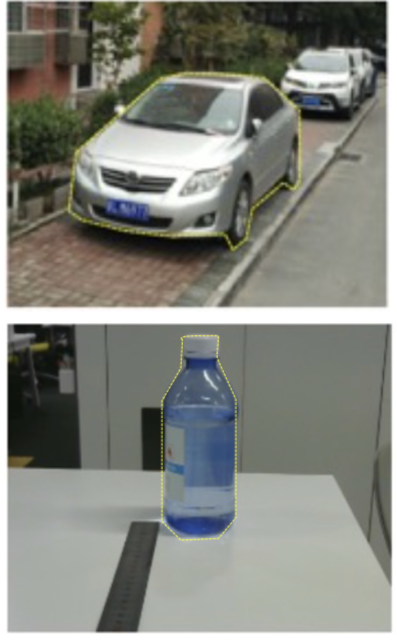
\includegraphics[width=.26664\textwidth]{translate/psgpaper_fig11}}
	\subcaptionbox{点云形式的重建结果}
	{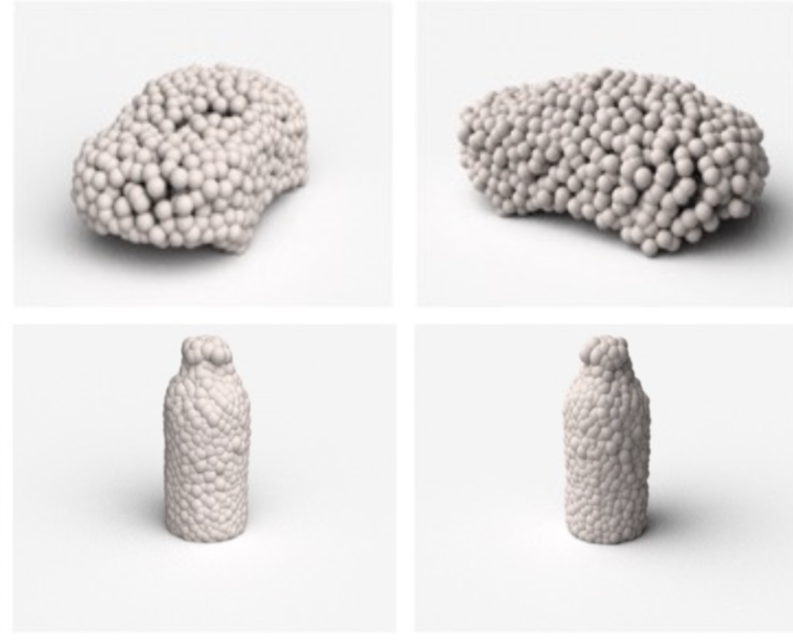
\includegraphics[width=.53328\textwidth]{translate/psgpaper_fig12}}
	\caption[]{
	本工作可以从单视角图像中,以点云的形式重建出{\heiti 完整}的三维物体。
	我们将重建结果从两个不同视角(沿方位角 $0^\circ$和 $90^\circ$)分别进行了展示。每个点都被视为一个小球体。Mask 用于指示图像中待重建物体的范围}
\end{figure}





在本文中,我们解决了基于单物体的单视角图像,
重建其三维几何结构的问题。
我们%基于
使用点云表示构建了三维几何形状的生成网络。
与使用
%几何图元或甚至简单网格的CAD模型相比
三角面片或者 CAD 原语相比,
点云在表示 % 底层的
连续的 三维 几何表面时可能不如前两者有效,但
% 出于我们的目的,
对与我们来说,它具有许多优点。
点云是简单且均匀的结构, 更容易被学习,因为它不需要编码多个 CAD 原语及其组合连接的模式。
此外,在涉及到几何变换和变形时,点云的处理方式更简洁,因为连接关系不需要更新。 我们的流水线架构根据输入图像和推断出的视角位置,预测出三维坐标中的各点位置。

由于采用了这种非常规的输出形式,
我们面临的挑战之一是如何衡量训练过程中的优劣。
注意到,相同的三维几何结构可能有不同的点云表示,然而它们在近似程度上相同的。
与通常的 $L_2$ %类
型%的
损失函数不同,
我们使用了传输问题中常见的 % 求解分问题的 % 常用的
% 基于
推土机距离 (Earth Mover's Distance, EMD) %的%运输问题的
%解决方案
,有效地解决了衡量训练结果优劣的问题。%分配问题 我们利用EMD的近似来提供速度,并确保端到端培训的可区分性。

我们的方法使用从训练数据集中学习到的先验知识,有效地解决了基于单视角图像三维重建
%恢复的不适合问题
的局限性问题。
网络必须估计输入图像可见部分的深度,并根据先验知识合理的补充出其余不可见几何对象的位置。
%评估几种不同完成的合理性。
从统计的角度来看,如果我们能够充分地提取出真实情况的特征,或者从具有不确定性的真实情况中采样,
%表征地面真实空间的景观,或者能够相应地抽样合理的候选人,
那将是非常理想的。
然而,一个比较独特而有趣的关键点在于,如果我们认为这是一个回归问题,
那么重建结果在某些视角%视图
中具有固有的多样性与不确定性。
在这样的情况下,同样的二维图像可能对应着多个同样正确且合理的三维 重建结果。
这使得我们的问题有别于每个训练样本都有唯一真实标注数据的经典回归、%问题与
分类问题。%设置
%有很大不同。 
% 在这种情况下,
因此,适当定义好损失函数,对于获得最有意义的重建结果至关重要。


% TODO 标点 ;。,: ;,.:sn
% ;,.:ok

我们的最终算法是一个条件采样器,它从给定输入图像中,估计出所有合理重建结果的概率分布,并从中采样出一个三维点云作为输出。
我们使用渲染合成出的图像以及现实世界中拍摄的图像进行了实验,验证了本文方法的有效性。
我们的贡献可以总结如下几点:
\begin{itemize}
	\item 我们首次通过深度学习的方法研究点集生成问题;
	\item 在基于单视角图像的 三维 重建任务中,我们提出了点云生成网络,且明显优于目前最先进的技术;
	\item 我们系统地探讨了点云生成网络的体系结构和损失函数的设计问题;
	\item 我们提出了一个经验性的方案,有效解决了单视角图像三维重建问题中的多样性和不确定性。
\end{itemize}









\section{相关工作}
 {\heiti 基于单视角图像的三维重建}
尽管大多数研究集中在多视角图像中的几何结构上,如 SFM\acite{[11]} 和 SLAM\acite{[10]}等,但理想情况下,人们更希望可以从丰富的单视角图像中重建三维物体的几何形态。

但是,在这样的需求和设定下,问题是受限制的。必须纳入有效的先验知识,问题才能被有效地加以解决。
早期的工作如 ShapeFromX \acite{[13,1]} 对三维物体形状和环境光照条件做出了强烈的假设。
{[12,21]} 开创了对简单几何结构使用基于学习的方法重建的先河。 图像集合中的粗略对应关系也可用于粗略的三维形状估计\acite{[15,3]}。
随着商用三维传感器的流行,RGB-D 数据库已经被构建,并用于训练基于机器学习的系统\acite{[7,9]}。
尽管我们取得了很大的进步,但这些方法仍然无法从单幅图像中稳定地重建出完整和高质量的图像,因为已有算法没有学习到更强大的几何先验知识。

最近,一些大型三维 CAD模型库,如 ShapeNet\acite{[4]} 等被提出。
他们有效地助力于解决三维重建任务,且有很大的潜力。
例如,文献 [22,14] 提出将现有形状变形并重新组装,形成与输入图像匹配的新模型。
这些系统依赖于高质量的图像形状匹配关系,而这本身同样是一个具有挑战性的问题。


更接近于我们的工作的是文献 [5]。
在 [5] 的工作中,他们使用神经网络,将给定图像中的三维模型以 体素的表示形式重建出来。 我们的工作和 [5] 相比,有两个关键区别:首先,[5] 中的重建结果是基于三维 体素表示的;而我们的重建结果基于点云表示。 正如我们在
第 \ref{section:translate:psg_reconrgb} 节中
所证明和分析的,点集为神经网络形成了一个更好的形状空间,因此重建结果的形状往往更加完整和自然。其次,对于单个输入图像,我们提供了多个候选的重建结果。这样的设计反映了单个图像不足以完全重建出物体三维形状
%重建
的事实。


{\heiti 基于深度学习的几何对象合成}
总体而言,如何以端到端的方式预测几何形状,还是一个有待探索的新课题。
%的领域是一个相当原始的土地。 
特别地,% 在本文中
我们的输出——三维点云,在深度学习社区中还不是典型的处理对象。一个点云包含来自度量空间的无序样本。因此,其等价类被定义为排列。此外,我们还必须考虑点云间的距离。 据我们所知,%我们并不知道
以前的深度学习系统并不能%能够
有效的生成、预测这些对象。






\section{问题定义与记号说明}
我们的目标是从单视角的二维 RGB 图像或 RGB-D 图像中重建出三维物体的完整形状。
我们以无序点集 $S = \{(x_i, y_i, z_i)\}^N_{i = 1}$的形式表示物体的三维重建结果,其中 $N$ 是预定义的常数。 我们观察到,对于大多数%使用的
%常用的
三维物体而言,使用  $N = \numprint{1024}$  足以保存其主要的几何结构。

点云的一个优势来自其无序性。 与深度图等基于二维图像的表示不同,拓扑约束不会%放在
出现在点云表示中。
与基于三维点阵的体素表示相比,点云可以通过仅编码曲面上的点,来获得更高的效率。
此外,坐标值 $(x_i, y_i, z_i)$ 需要旋转或缩放时,仅仅需要经过简单的线性变换即可实现目标,这与体素表示的情况形成鲜明对比。

为了对问题的不确定性进行建模,我们将真实的重建结果定义为以输入图像 $\bm I$ 为条件的概率分布 $p(\cdot | \bm I)$。在训练时,对于数据集中的每幅图像,我们只能获得一个合理的三维重建结果,即概率分布 $p(\cdot | \bm I)$ 中的一个样本。

我们训练神经网络 $G$,作为概率分布 $P(\cdot | \bm I)$ 的条件采样器:
\begin{align}
	S = G(\bm I, \bm r; \bm \theta) \tag*{\ref{chap:translate}-1} \label{eq:translate:psg_network}
\end{align}
其中 $\bm \theta$ 表示网络参数,$\bm r \sim \NormDist(\bm 0, \bm I)$ 是扰乱输入的随机变量
\footnote{类似于条件生成对抗网络 (Conditional Generative Adversarial Network, CGAN)\acite{[17]}。}。
在测试期间,我们可以使用随机变量 $\bm r$ 的多个采样样本来生成不同的重建结果。















\section{方法}
\subsection{概览}

由于点云表示的无序性以及重建结果中固有的多样性和不确定性
,我们设计点云条件生成网络的任务充满了挑战。
这些挑战促使我们发明新的网络架构,损失函数以及%学习
训练方法。
具体而言,我们必须解决以下三个子问题:
\begin{itemize}
	\item {\heiti 点云生成结构}:
	      预测点集的神经网络在已有的文献中几乎没有研究,为我们的探索和设计留下了巨大的
	      %开放
	      选择空间。
	      理想情况下,点云生成网络应充分利用训练数据的统计规律,并拥有足够强大的表示能力。
	      我们提出了一个具有两个预测分支的网络架构,
	      一个在捕捉复杂几何结构方面具有高度灵活性,
	      另一个巧妙地利用几何连续性粗略地预测出三维物体的轮廓。
	      它的表达能力可以通过 hourglass 结构得到进一步的加强。
	      具体细节请参见第 \ref{section:translate:psg_gen} 节
	      。


	\item {\heiti 比较点集差异的损失函数}:
	      对于我们的新提出的三维表示形式——点云,目前还不清楚如何衡量预测结果和真实结果之间的差距。我们为点集引入了两个距离度量——Chamfer 距离 (Chamfer Distance, CD) 和 推土机距离 (Earth Mover's Distance, EMD)。
	      我们证明了两个距离度量几乎在任何地方都是可微的,因此可以用作损失函数。但是,它
	      们在捕捉几何形状时具有不同的特性。
	      具体细节请参见第 \ref{section:translate:psg_loss} 节。




	\item {\heiti 刻画重建结果的多样性与不确定性}:
	      基于单视角图像恢复物体三维结构是一个受限制的问题,
	      因为在训练和测试时,真实的重建结果有一定的多样性和不确定性。
	      对于一个给定的输入,有效的表示出此不确定性非常重要。此外,在实际使用中,我们更希望能够基于这样的不确定性产生多个合理的预测。
	      令人惊讶的是,这个目标可以通过简单地使用 $\min$函数对我们已经提出的损失函数进行包装,或者通过条件变分自编码器 (Conditional Variational Autoencoder, CVAE) 来巧妙地实现。具体细节请参见第 \ref{section:translate:psg_uncertainty} 节。

\end{itemize}

\subsection{点云预测网络 \label{section:translate:psg_gen}}
设计点云预测网络是一个全新的任务。
我们精心设计了一个点云生成网络,为复杂几何结构提供了强大的网络表达能力,并使得网络能够充分利用已知训练数据的几何统计规律。
为了逐步介绍我们的网络,我们从一个简单的版本开始,逐步添加组件。

\begin{figure}[h]
	\centering%
	\subcaptionbox{基本版\label{fig:translate:vanillapointsetgen}}
	{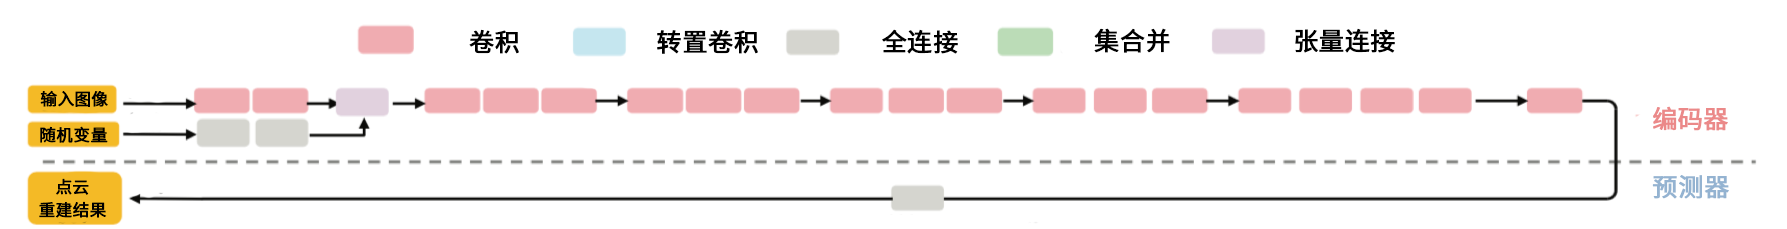
\includegraphics[width=.999\textwidth]{vanillapointsetgen}}
	\\

	\subcaptionbox{双分支版\label{fig:translate:tbpointsetgen}}
	{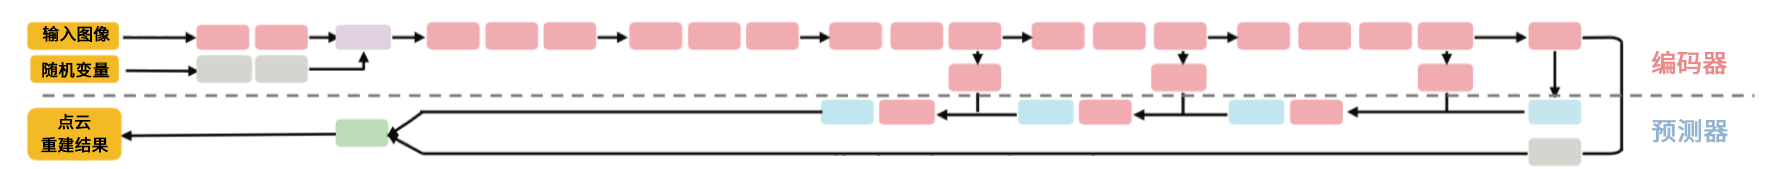
\includegraphics[width=.999\textwidth]{tbpointsetgen}}
	\\

	\subcaptionbox{Hourglass 版 \label{fig:translate:hpointsetgen}}
	{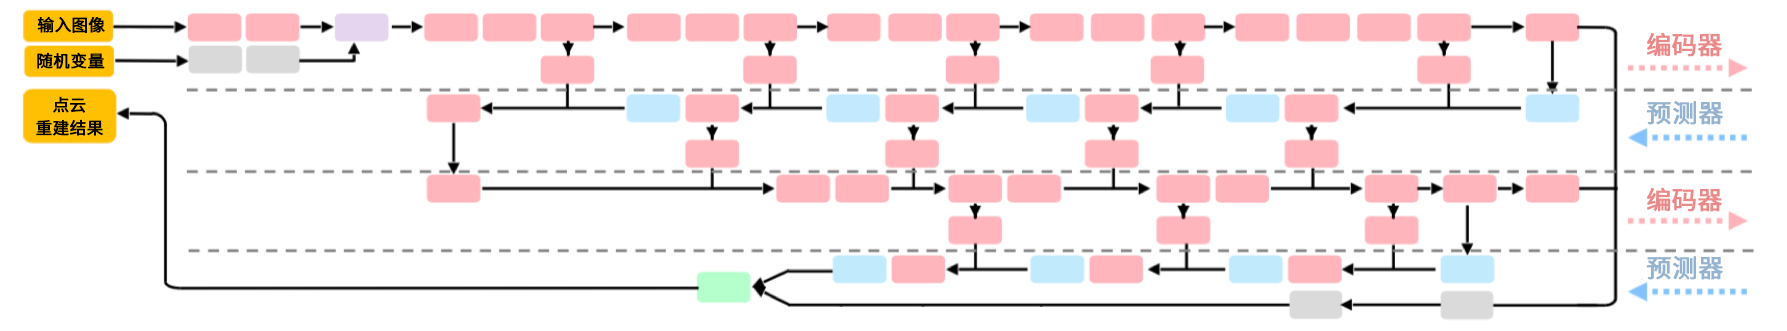
\includegraphics[width=.999\textwidth]{hpointsetgen}}
	\\
	\caption[]{
		点云生成网络的结构} \label{fig:translate:genpointsetgen}
\end{figure}

如图 \ref{fig:translate:vanillapointsetgen} 所示,我们的网络可被分为编码器和预测器两部分。 编码器将输入图像 $\bm I$ 和随机向量 $\bm r$ 映射到隐空间中,
而预测器进一步将中间表示映射为重建结果,并以 $N \times 3$ 的矩阵 $\bm M$ 表示,其中每行包含一个点的坐标。

编码器是卷积层和 线性整流单元 (Rectified Linear Unit, ReLU) 的组合。此外,它还包括了一个随机向量 $\bm r$ 的输入,以增强输入图像 $\bm I$ 重建结果的多样性。
我们将把随机变量 $r$ 的作用和使用方法推迟到第 \ref{section:translate:psg_uncertainty} 节来详细解释。 预测器通过全连接网络回归出 $N$ 个点的三维坐标。 虽然此版本的设计很简单,但它在实践中表现得相当好。

我们进一步改进了预测分支的设计,以更好地适应常见自然物体中的%大而
光滑表面。上文中介绍的全连接预测器不足以充分利用这种自然几何表面的统计规律,因为每个点都是独立预测的。
图 \ref{fig:translate:tbpointsetgen} 所示的改进预测器进一步利用了几何表面的光滑性。

该版本具有两个并行的预测器分支:全连接 (Fully Connected, FC) 分支和转置卷积 (Deconvolution, Deconv) 分支。
全连接分支与基本版相比没有变化,同样预测 $N_1$ 个点。
而转置卷积分支预测尺寸为 $H \times W$的三通道图像,其中每个像素的三个通道值是点的坐标,即此分支提供另外 $H \times W$ 个点。
最后,它们的预测结果被合并到一起,形成了共计 $N = N_1 + H \times W$ 个点的最终结果。
此外,我们还加入了多个跨层连接 (Skip Link) 来增强编码器和预测器间的信息传递。


通过 全连接 分支,我们的模型具有很高的灵活性。
它在描述错综复杂的几何结构时表现出了良好的性能。 通过 转置卷积 分支,我们的模型不仅可以通过权值共享实现更多参数节省, 而且更容易生成光滑的表面,因为卷积和转置卷积操作的在空间上连续性。
第 \ref{section:translate:net_analyse} 节中的实验结果更好地佐证了上述结论。


为了追求更好的性能,我们引入了 hourglass 版本,如图 \ref{fig:translate:hpointsetgen} 所示。它的灵感来自于文献 [18]。
这个深度神经网络反复进行编解码操作,因此具有更强的表示能力,能更好地综合全局信息和局部信息。

上面介绍了式 \eqref{eq:translate:psg_network} 中网络 $G$ 的设计。然而,为了训练这个网络,我们仍然需要为点云重建结果设计适当的损失函数,并使得 $r$ 能够合理刻画重建结果的多样性和不确定性,让网络能够预测出多个合理的结果。
我们将在接下来的两节中详细说明%解释% 损失函数的设计以及不确定性的刻画。
%如何设计损失函数并刻画重建结果的不确定性。
。



\subsection{点集之间的距离度量 \label{section:translate:psg_loss}}
设计一个好的损失函数来比较预测的点云和实际情况,是一个重要的挑战。 为了能够融入已有的深度神经网络,合适的损失函数必须满足以下三个条件:
\begin{enumerate}
	\item 相对于点位置可微;
	\item 可被高效计算,因为数据将被多次前向和反向传播;
	\item 对集合中少数异常点具有鲁棒性(例如,Hausdorff 距离不能被采纳)。
\end{enumerate}

我们需要定义 $\mathbb{R}^3$ 各子集之间的距离函数 $d$,使得损失函数
$\Loss\left(\{S_i^{\text{pred}}\}, \{S_i^{\text{gt}}\}\right)$
能使用下面的形式:
\begin{align}
	\Loss\left(\{S_i^{\text{pred}}\}, \{S_i^{\text{gt}}\}\right)
	= \sum d\left(S_i^{\text{pred}}, S_i^{\text{gt}}\right)
	\tag*{\ref{chap:translate}-2} \label{eq:translate:psg_loss}
\end{align}
其中 $i$ 是数据点的编号,$S_i^{\text{pred}}, S_i^{\text{gt}}$ 分别是各个数据的预测结果和真实点云。

我们提出两个候选的度量方案:Chamfer 距离 (Chamfer Distance, CD) 和 推土机距离 (Earth Mover's Distance, EMD)\acite{[20]}。


\begin{itemize}
	\item {\heiti Chamfer 距离}:
	      我们定义两点集 $S_1, S_2 \subseteq \mathbb{R}^3$ 之间的 Chamfer 距离为:
	      \begin{align}
		      \DCD{S_1}{S_2} & =
		      \sum_{\bm x \in S_1} 􏰘\min_{\bm y \in S_2} \Norm*{\bm x - \bm y}^2 +
		      \sum_{\bm y \in S_2} 􏰘\min_{\bm x \in S_1} \Norm*{\bm x - \bm y}^2
		      \notag
	      \end{align}
	      %从严格意义上说,
	      严格地说,Chamfer 距离不是一个距离函数,因为三角不等式不成立。但是,我们仍然使用术语“距离”来指代任何在两个点集上定义的非负函数。
	      对于点集中的每个点,算法会找到另一个集合中的最近邻点,并将其平方距离累加求和。%加起来。 
	      如果 将 Chamfer 距离 视为定义在集合 $S_1$ 和 $S_2$ 中各点坐标上的函数,那么 $\DCD{\cdot}{\cdot}$是连续且分段光滑的。由于每个点的搜索过程是独立的,因此算法可以很容易地并行化。 而且,像 $k$-d 树这样的空间数据结构可以用来加速最近邻搜索的过程。
	      虽然 Chamfer 距离很简单,但它在实践中足以产生合理的高质量结果。


	\item {\heiti 推土机距离}:
	      考虑两个同基数的点集合 $S_1, S_2 \subseteq \mathbb{R}^3$,其中基数 $s = |S_1| = |S_2|$。$S_1, S_2$ 之间的推土机距离被定义为:
	      \begin{align}
		      \DEMD{S_1}{S_2} =
		      \min_{ \phi:\, S_1 \to S_2} \sum_{\bm x \in S_1} \Norm*{\bm x - \phi(\bm x)}_2
		      \notag
	      \end{align}
	      其中 $\phi:\, S_1 \to S_2$ 是一个双射。

	      推土机距离解决了一个优化问题,即分配问题。
	      对于除了零测度子集以外的几乎所有点集合对,在点的无限小移动下,
	      最优双射 $\phi$ 是唯一且固定的。 因此,EMD 几乎处处可微。
	      然而,对于实践中的深度学习而言,推土机距离的精确计算非常耗费资源,即使我们使用了图形硬件进行加速。
	      因此,我们采用了由文献 [2] 给出的 $(1 + \epsilon)$ 近似方案。 我们为每次测试分配了固定的运行时间,并逐步调整允许的错误率以确保计算得以终止。 对于典型的输入,该推土机距离的求解算法给出了高度准确的结果,近似误差可被控制在 $1 \%$ 内。
	      此外,该算法很容易在 GPU 上并行化。
\end{itemize}

{\heiti 几何形状空间}
尽管深度神经网络有强大的表达能力,但它在预测三维物体的精确几何形状时,会不可避免地会受到不确定性影响。 这种不确定性可能是由于网络容量有限、输入所采用的分辨率不足以及三维到二维投影过程中深度信息丢失导致的歧义。
面对无法精确解析形状的内在不足,神经网络倾向于预测所有可能形状的“均值”。而这样的均值形状具有所使用距离函数的本质特征。


\begin{figure}[h]
	\centering%
	\renewcommand{\tabularxcolumn}[1]{>{\arraybackslash} m{#1}}
	\begin{tabular}{ccccc}
		输入图像                                                 &
		\cincludegraphics[width=.15\textwidth]{translate/mean1}  &
		\cincludegraphics[width=.15\textwidth]{translate/mean2}  &
		\cincludegraphics[width=.15\textwidth]{translate/mean3}  &
		\cincludegraphics[width=.15\textwidth]{translate/mean4}    \\
		\begin{tabular}{@{}c@{}} 推土机距离的\\均值化结果 \end{tabular}                               &
		\cincludegraphics[width=.15\textwidth]{translate/mean5}  &
		\cincludegraphics[width=.15\textwidth]{translate/mean6}  &
		\cincludegraphics[width=.15\textwidth]{translate/mean7}  &
		\cincludegraphics[width=.15\textwidth]{translate/mean8}    \\
		\begin{tabular}{@{}c@{}} Chamfer 距离的\\均值化结果 \end{tabular}                               &
		\cincludegraphics[width=.15\textwidth]{translate/mean9}  &
		\cincludegraphics[width=.15\textwidth]{translate/mean10} &
		\cincludegraphics[width=.15\textwidth]{translate/mean11} &
		\cincludegraphics[width=.15\textwidth]{translate/mean12}   \\
		                                                         &
		\begin{minipage}[b]{.15\textwidth}
			\subcaption{}\label{fig:translate:mean_a}
		\end{minipage}                               &
		\begin{minipage}[b]{.15\textwidth}
			\subcaption{}\label{fig:translate:mean_b}
		\end{minipage}                               &
		\begin{minipage}[b]{.15\textwidth}
			\subcaption{}\label{fig:translate:mean_c}
		\end{minipage}                               &
		\begin{minipage}[b]{.15\textwidth}
			\subcaption{}\label{fig:translate:mean_d}
		\end{minipage}                                 \\
	\end{tabular}

	\caption[]{
		推土机距离和 Chamfer 距离的均值化结果。
		几何形状的分布分别是
		\subref{fig:translate:mean_a}
		半径变化的圆形;
		\subref{fig:translate:mean_b}
		沿对角线移动的尖刺圆弧;
		\subref{fig:translate:mean_c}
		在矩形条周围的其中一个角上随机分配的一个方形;
		\subref{fig:translate:mean_d}
		竖条旁边以 $0.5$ 概率出现的一个圆盘。
		红点表示相应地根据推土机距离和 Chamfer 距离计算出的均值化形状} \label{fig:translate:mean}
\end{figure}




在图 \ref{fig:translate:mean} 中,我们通过随机梯度下降算法最小化 $\EXPECT{s \sim S}{\left[\Loss(x, s)\right]}$ ,用于说明在我们构造的几何形状分布上,推土机距离和 Chamfer 距离均值化结果的区别,其中 $S$ 是给定的几何形状分布,$\Loss$ 是两个距离函数之一。

在第一种情况和第二种情况下,存在单个连续变化的隐藏变量:
图 \ref{fig:translate:mean_a} 中的圆的半径和
图 \ref{fig:translate:mean_b} 中的尖刺圆弧的位置。 推土机距离可以粗略地捕捉与隐藏变量的平均值对应的形状。
相比之下,Chamfer 则得出了一种飞溅的形状,破坏了原有的几何形状和结构。 在后两种情况下,存在离散变化的隐藏变量:
图 \ref{fig:translate:mean_c} 中方块位于哪个角落,
以及图 \ref{fig:translate:mean_d} 中除竖条之外是否还有圆。 为了解决变化部分是否存在及其位置的不确定性,最小化 Chamfer 距离可以使得均值化的结果在主体部分之外分配一些位置正确的点;而最小化推土机距离则存在显著的失真。




\subsection{生成多种可能的重建结果 \label{section:translate:psg_uncertainty}}

我们的算法需要求解基于单视角图像三维重建的局限性问题。
作为一个回归问题,预测结果的多样性和不确定性常常出现,例如在测试阶段,可见部分的深度不能够直接确定,而不可见部分的几何形状必须通过猜测的方式补充完整。
从统计的角度来看,输入图像的所有合理预测形成了一个概率分布。
这意味着在训练集中,两张看起来相似的图像可能具有
%相当不同
差异很大的真实重建结果。重申我们在前一节中的讨论:真实情况的不确定性可能会显着影响训练出的预测器,
% 因为损失函数
因为损失函数 \eqref{eq:translate:psg_loss} 会导致我们的模型倾向于预测出所有合理重建结果的平均值。


为了更好地刻画重建结果的不确定性或输入图像中固有的歧义,例如单视角图像中看不见的部分,
我们希望系统能够按照所有重建结果的分布进行采样,得到最终的输出结果。
我们期望将一个随机变量 $r$ 传递给网络 $G$,如式 \eqref{eq:translate:psg_network} 所示。
这将有助于网络探索真实重建结果的分布,类似于条件生成对抗网络
(Conditional Generative Adversarial Network, CGAN) \acite{[17]}。
然而,直接将 \eqref{eq:translate:psg_network} 中的 $G$ 代入损失函数
\eqref{eq:translate:psg_loss} 来预测 $S_i^{\text{pred}}$
%进入损失(2)来预测Spred将不起作用,因为损失i
并没有效果,因为最小化损失函数将使随机变量 $r$ 无法发挥作用。
目前还不清楚如何如何使用条件生成对抗网络求解我们的问题,因为如何构造一个直接能处理点集的判别器,还是一个有待研究的开放问题。

这个问题可以通过 VAE 等更复杂的框架来解决,这是的我们可以对网络增加一个输入通道,例如另一个视角的图像等。
但是,我们找了一种在实际应用中更简单而有效的不确定性建模方法:最小 $n$ 损失函数 (Min-of-N loss, MoN loss)。我们通过最小化以下损失函数:
\begin{align}
	\Loss(\bm \theta) = \sum_k
	\min_{\substack{\bm r_j \sim \NormDist(\bm 0, \bm I) \\  1 \le j \le n}}
	d\left(
	{G(I_k, \bm r_j; \bm \theta)    }
	,
	{   S_k^{\text{gt}}   }
	\right)
	\tag*{\ref{chap:translate}-3} \label{eq:translate:psg_mon}
\end{align}
来训练我们的网络。

我们在此简要说明最小 $n$ 损失函数 \eqref{eq:translate:psg_mon} 的基本原理。给定图像 $\bm I_k$,
$G$ 通过 $n$ 个随机向量 $\bm r_j$ 的扰动输入,来预测出 $n$ 个点的位置。
直觉上,我们期望
所有预测结果中的某一个将接近于训练数据中给出的真实情况 $S_k^{\text{gt}}$,
% 通过训练数据,
这意味着每个预测结果与真实情况之间 $n$ 个距离的最小值必须很小。



\begin{figure}[h]
	\centering
	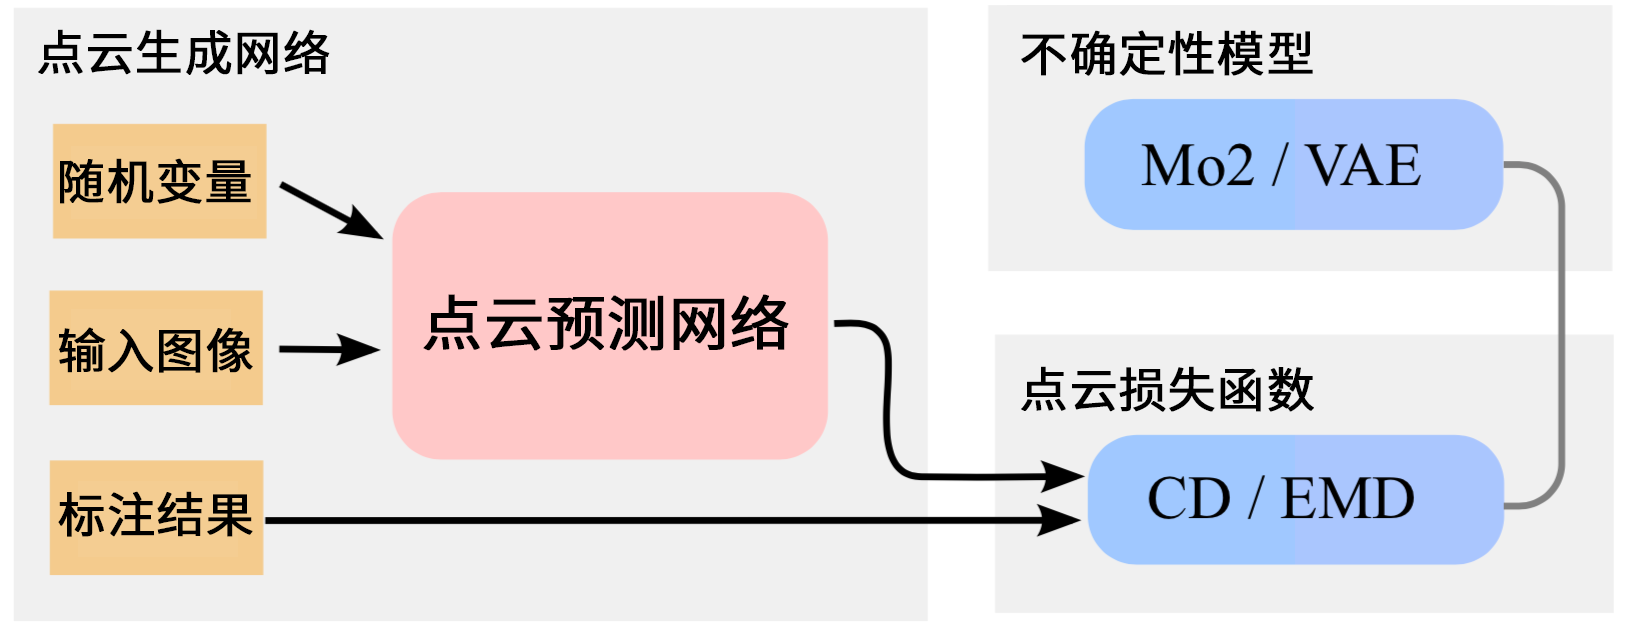
\includegraphics[width=.6\textwidth]{translate/pipe}
	\caption[]{
		系统结构。
		通过不确定性模型,我们的系统能够生成多个重建结果}
	\label{fig:translate:pipe}
\end{figure}



我们将此损失函数命名为最小 $n$ 损失函数,因为它是 $n$ 个距离的最小值。
图 \ref{fig:translate:genpointsetgen} 中的所有点云生成网络都可以与 图 \ref{fig:translate:pipe} 中的最小 $n$ 损失函数相互整合。
在实践中,我们发现:只需令 $n = 2$,算法就已经能够把握真实重建结果的概率分布。
详细的实验结果请参见第 \ref{section:translate:net_multi} 节。

\begin{figure}[h]
	\centering
	\includegraphics[width=.9\textwidth]{translate/VAE}
	\caption[]{
		作为几何形状采样器 $p(S | X)$ 的条件变分自编码器的网络架构。 左图:训练阶段的条件变分自编码器,可通过前馈神经网络实现。
		其中,$Y$ 是真实三维形状 $S$ 的体素表示形式,而 $f(z, X)$是对于 $S$所预测出的点云重建结果。右图:测试阶段的同一条件变分自编码器。本图是根据文献 Doersch et al. [6] 修改而成的}
	\label{fig:translate:vae}
\end{figure}

实现条件采样器的另一种方法是使用条件变分自编码器。 有关变分自编码器的更多详细信息,请参见文献 [6]。
图 \ref{fig:translate:vae}
显示了我们的在训练和测试阶段所采用的条件变分自编码器 $p(S | X)$ 的系统架构。其中,$X$ 是输入图像,$S$ 是三维物体的真实点云表示。
在训练时,每个输入图像 $X$ 将被一个受 $Y$ %为条件
控制的随机变量所增强,其中 $Y$ 是真实形状 $S$ 的体素表示。
我们使用了三维卷积神经网络作为编码器 $Q$。关于三维卷积神经网络的细节,请参见文献 [16]。 因此,在隐空间中的某个局部内,包含着所有可能的三维重建结果。











\section{实验}
\subsection{通过渲染生成训练数据}


首先,我们介绍如何准备训练数据。 我们采用核心方法是对 CAD 模型进行渲染,从而到其对应视角的二维图像。
我们所用的模型来自 ShapeNet 数据集\acite{[4]}。它包含大量经人工手动校正的三维模型及其纹理。
具体而言,我们仅仅使用了其中 \numprint{220 000} 个三维模型,涵盖了 \numprint{2000} 个类别。
现有的一些研究成果 \acite{[5,19]}%已经采用了
%曾经
也采用过通过渲染合成出的数据来训练神经网络。

对于每个模型,我们将其外接半球半径归一化为单位 $1$,并将其地平面对齐。 然后,我们根据 Blinn-Phong 光照模型,随机选择环境贴图,将每个模型渲染成二维图像。 在我们的实验中,为了节省计算时间,我们使用了简单的局部照明模型。
但事实上,我们的方法%同样
显然可以扩展到全局照明算法和更复杂的背景上。%这样的改进是很直观的。



\subsection{基于 RGB 图像的三维重建 \label{section:translate:psg_reconrgb}}


{\heiti 与最先进的技术进行比较}
我们将我们的工作与
目前所有基于深度学习的 三维 重建技术中最顶尖、最先进的
\threedrsns
\acite{[5]} 工作进行了比较。
\threedrsns
将单视角或多视角图像中的三维物体重建为体素表示。
为了进行比较,我们使用 \threedrsns 工作所采用的数据集重新训练了我们的网络。 我们将把两者的结果在三个不同的指标——Chamfer 距离、推土机距离和交并比 (Intersection over Union, IoU) 下进行比较。
在 \threedrsns 工作中,仅有 交并比 值被计算并记录,因此我们使用由原作者提供的预训练网络来进行其他指标的计算。
为了计算 Chamfer 距离、推土机距离,体素表示的重建结果及其真实结果
必须通过最远点采样 \acite{[8]} 算法,才能够得到与本工作具有相同的基数 $N = 1024$ 的离散点云。
在计算 交并比 时,我们需要将点云进行后处理,得到与 \threedrsns 工作
中相同分辨率的体素表示。有关后处理的详细信息,请参阅第 \ref{section:translate:psg_detail} 节。

\begin{figure}[h]
	\centering
	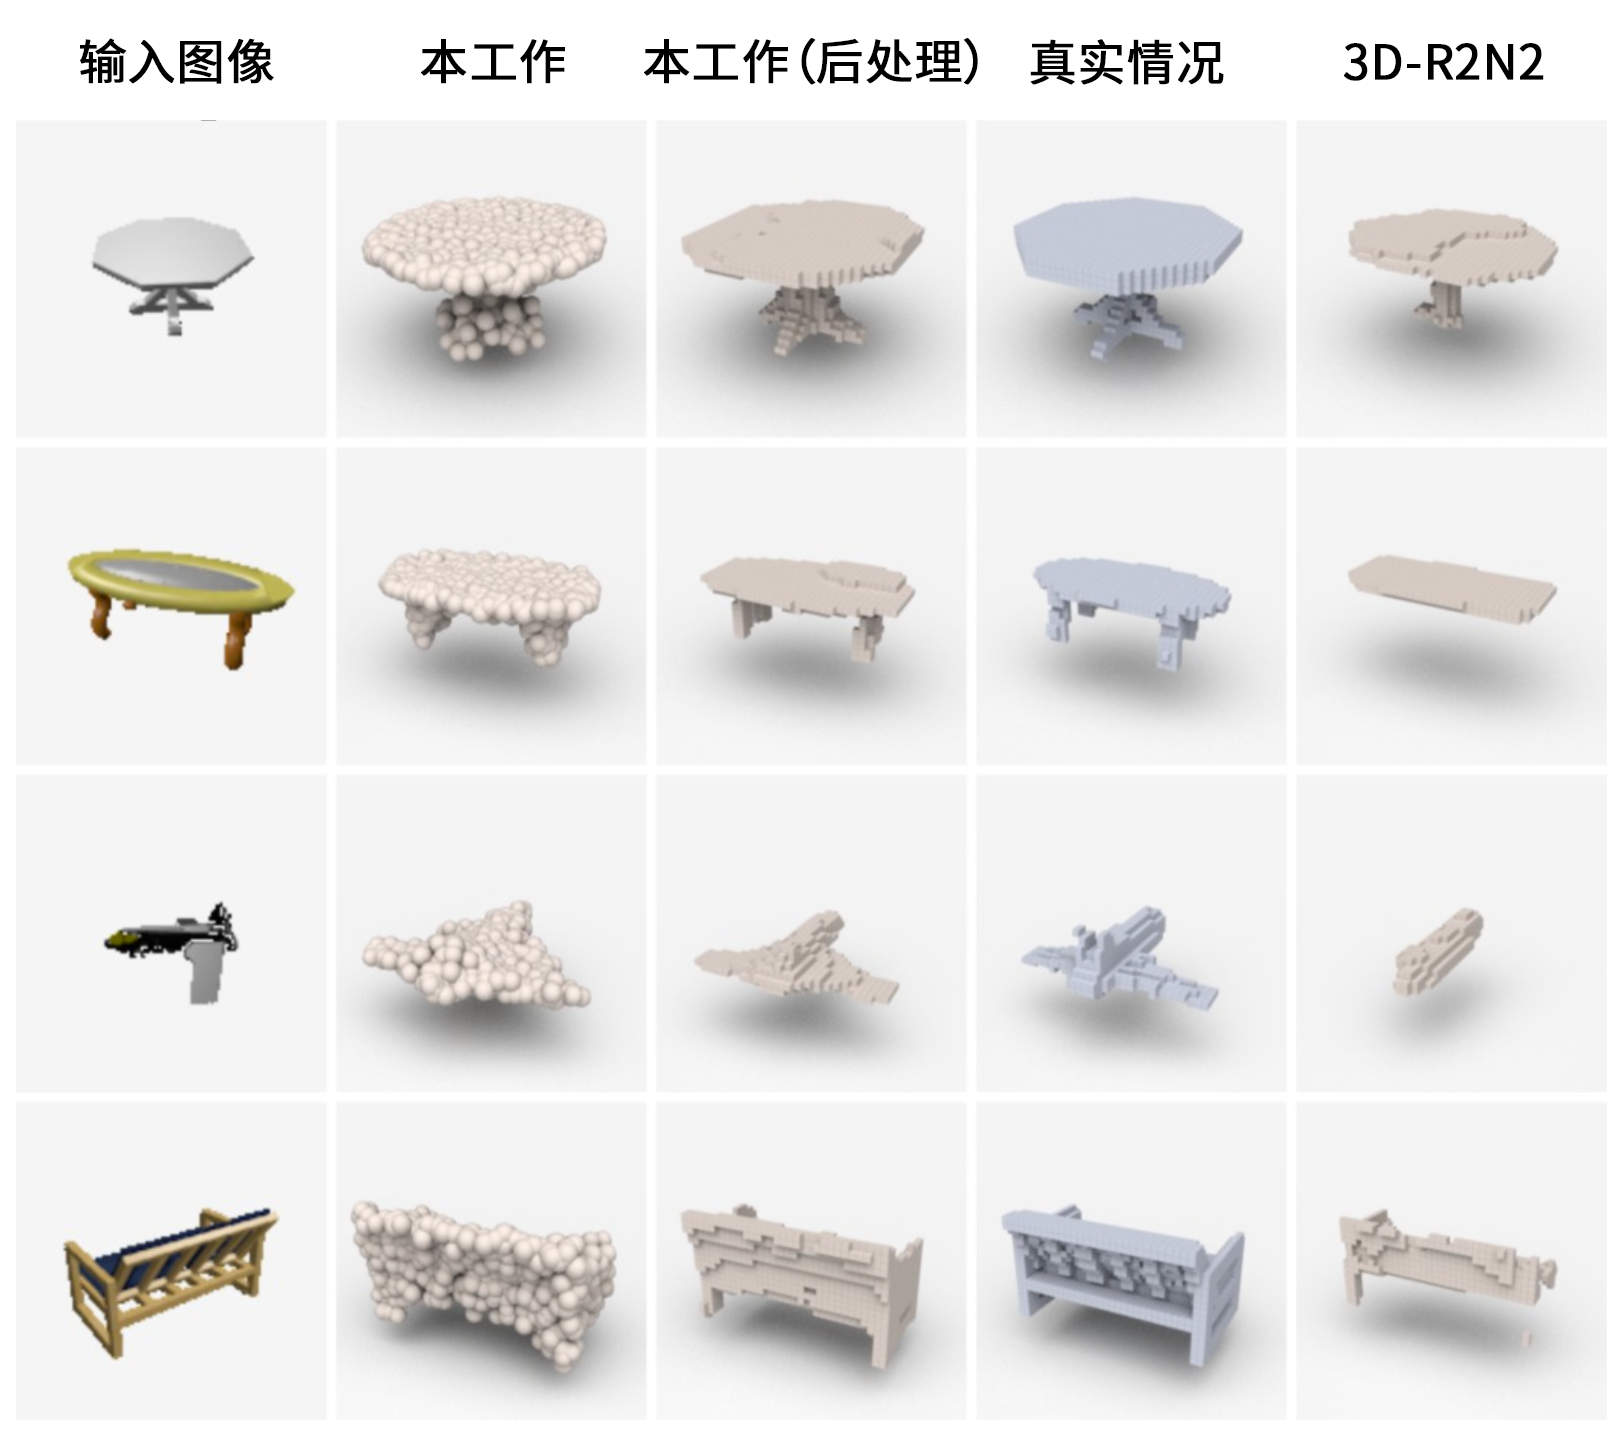
\includegraphics[width=.8\textwidth]{translate/cmp}
	\caption[]{与 \threedrsns 的可视化比较。我们的方法更好地保留了对象的细微几何结构}
	\label{fig:translate:cmp}
\end{figure}

\begin{figure}[h]
	\centering
	\hfill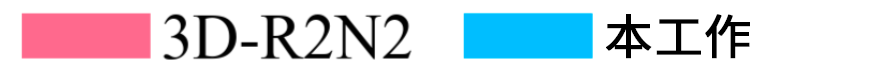
\includegraphics[width=.3\textwidth]{translate/cmp0}\\
	\subcaptionbox{\label{fig:translate:cmpqcdemd}}
	{
		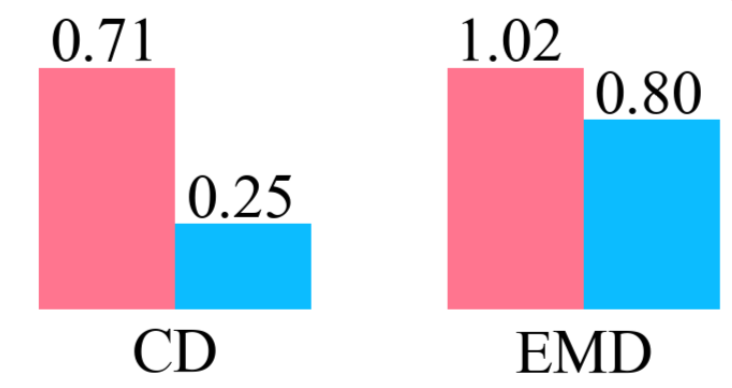
\includegraphics[width=.3\textwidth]{translate/cmp1}
	}
	\hspace{2em}
	\subcaptionbox{\label{fig:translate:cmpqiou}}
	{
		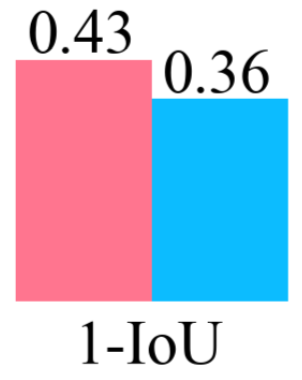
\includegraphics[width=.12\textwidth]{translate/cmp2}
	}
	\caption[]{与 \threedrsns 的定量比较。
		\subref{fig:translate:cmpqcdemd} 基于点云的 Chamfer 距离和推土机距离两项指标;
		\subref{fig:translate:cmpqiou} 基于体素表示的 $1 - \text{交并比}$指标。 数值越低表示错误较小。我们的方法在所有的三个指标上都有更好的结果}
	\label{fig:translate:cmpq}
\end{figure}

在图 \ref{fig:translate:cmpq} 中,
我们展示了%我们的网络
本工作与单视角 \threedrsns 相对比的结果。
为了确定 Chamfer 距离、推土机距离的绝对比例,我们将单位 1 定义成
在 \threedrsns 所用数据集中,用于表示真实重建结果的三维网格之边长的 $1/10$。 虽然没有直接通过交并比训练网络,但我们的网络在所有三项指标下都有显着提升。

\begin{table}[h]
	\centering
	\caption[]{各类别的三维重建结果的定量比较。 注意到在单视角的重建任务中,我们在所有类别上都实现了更高的交并比指标。 平均值是指各类别中指标的平均。 对于所有的 13 个类别中的 8 个,我们的结果甚至比 \threedrsns 已知五个视角图像的情况要更优}
	\label{tab:translate:cmp}
	\begin{tabular}{lcccccc}
		\toprule[1.5pt]
		\multirow{2}{*}{类别} &  & 本工作         &  &
		\multicolumn{3}{c}{\threedrsns}
		\\
		\cline{3-3} \cline{5-7}
		                      &  & 单视角         &  & 单视角 & 三视角 & 五视角
		\\
		\midrule[1pt]
		飞机                  &  & \textbf{0.601} &  & 0.513  & 0.549  & 0.561          \\
		长椅                  &  & \textbf{0.550} &  & 0.421  & 0.502  & 0.527          \\
		储藏柜                &  & 0.771          &  & 0.716  & 0.763  & \textbf{0.772} \\
		汽车                  &  & 0.831          &  & 0.798  & 0.829  & \textbf{0.836} \\
		椅子                  &  & 0.544          &  & 0.466  & 0.533  & \textbf{0.550} \\
		显示器                &  & 0.552          &  & 0.468  & 0.545  & \textbf{0.565} \\
		台灯                  &  & \textbf{0.462} &  & 0.381  & 0.415  & 0.421          \\
		扬声器                &  & \textbf{0.737} &  & 0.662  & 0.708  & 0.717          \\
		枪支                  &  & \textbf{0.604} &  & 0.544  & 0.593  & 0.600          \\
		长椅                  &  & \textbf{0.708} &  & 0.628  & 0.690  & 0.706          \\
		桌子                  &  & \textbf{0.606} &  & 0.513  & 0.564  & 0.580          \\
		手机                  &  & 0.749          &  & 0.661  & 0.732  & \textbf{0.754} \\
		船                    &  & \textbf{0.611} &  & 0.513  & 0.596  & 0.610          \\
		\hline
		平均值                &  & \textbf{0.640} &  & 0.560  & 0.617  & 0.631          \\
		\bottomrule[1.5pt]
	\end{tabular}
\end{table}


我们根据文献 [5] 形式,记录了本工作在每类物体上的交并比值。 从表 \ref{tab:translate:cmp} 中可以看出,对于单视角重建,我们所提出的方法在所有类别中都有着更高的交并比。
虽然 \threedrsns 还能够从多个视角的图像中预测更加精确的三维形状,
但是我们提出的基于单视角的方法在许多类别中甚至已经超过了 \threedrsns 在已知 5 个视角图像时的预测。

为了进一步对比这两种方法,我们可以看到一些典型的例子。 正如文献 [5] 所述,他们的方法经常会遗漏物体的细微特征,例如家具的腿等。
我们推测,这是由于 \threedrsns 所采用的体素表示形式
%和体素方面的
及其损失函数导致的。
它们不足以适当地调整这些细微几何结构的错位。
相反,我们基于点云的目标函数鼓励网络保留更精细的几何形状,
并使得我们的预测在结构上更合理。




\subsection{基于 RGB-D 图像的三维重建}

有趣的是,我们的方法的可以很容易地将额外的输入信息引入到重建系统中。 例如,把神经网络的输入变为 RGB-D 形式的图像,即引入深度信息时,
我们的重建系统就转变成了一个 三维 形状补全工具。 图 \ref{fig:translate:complete} 提供了三维形状补全的可视化结果。


\begin{figure}[h]
	\centering
	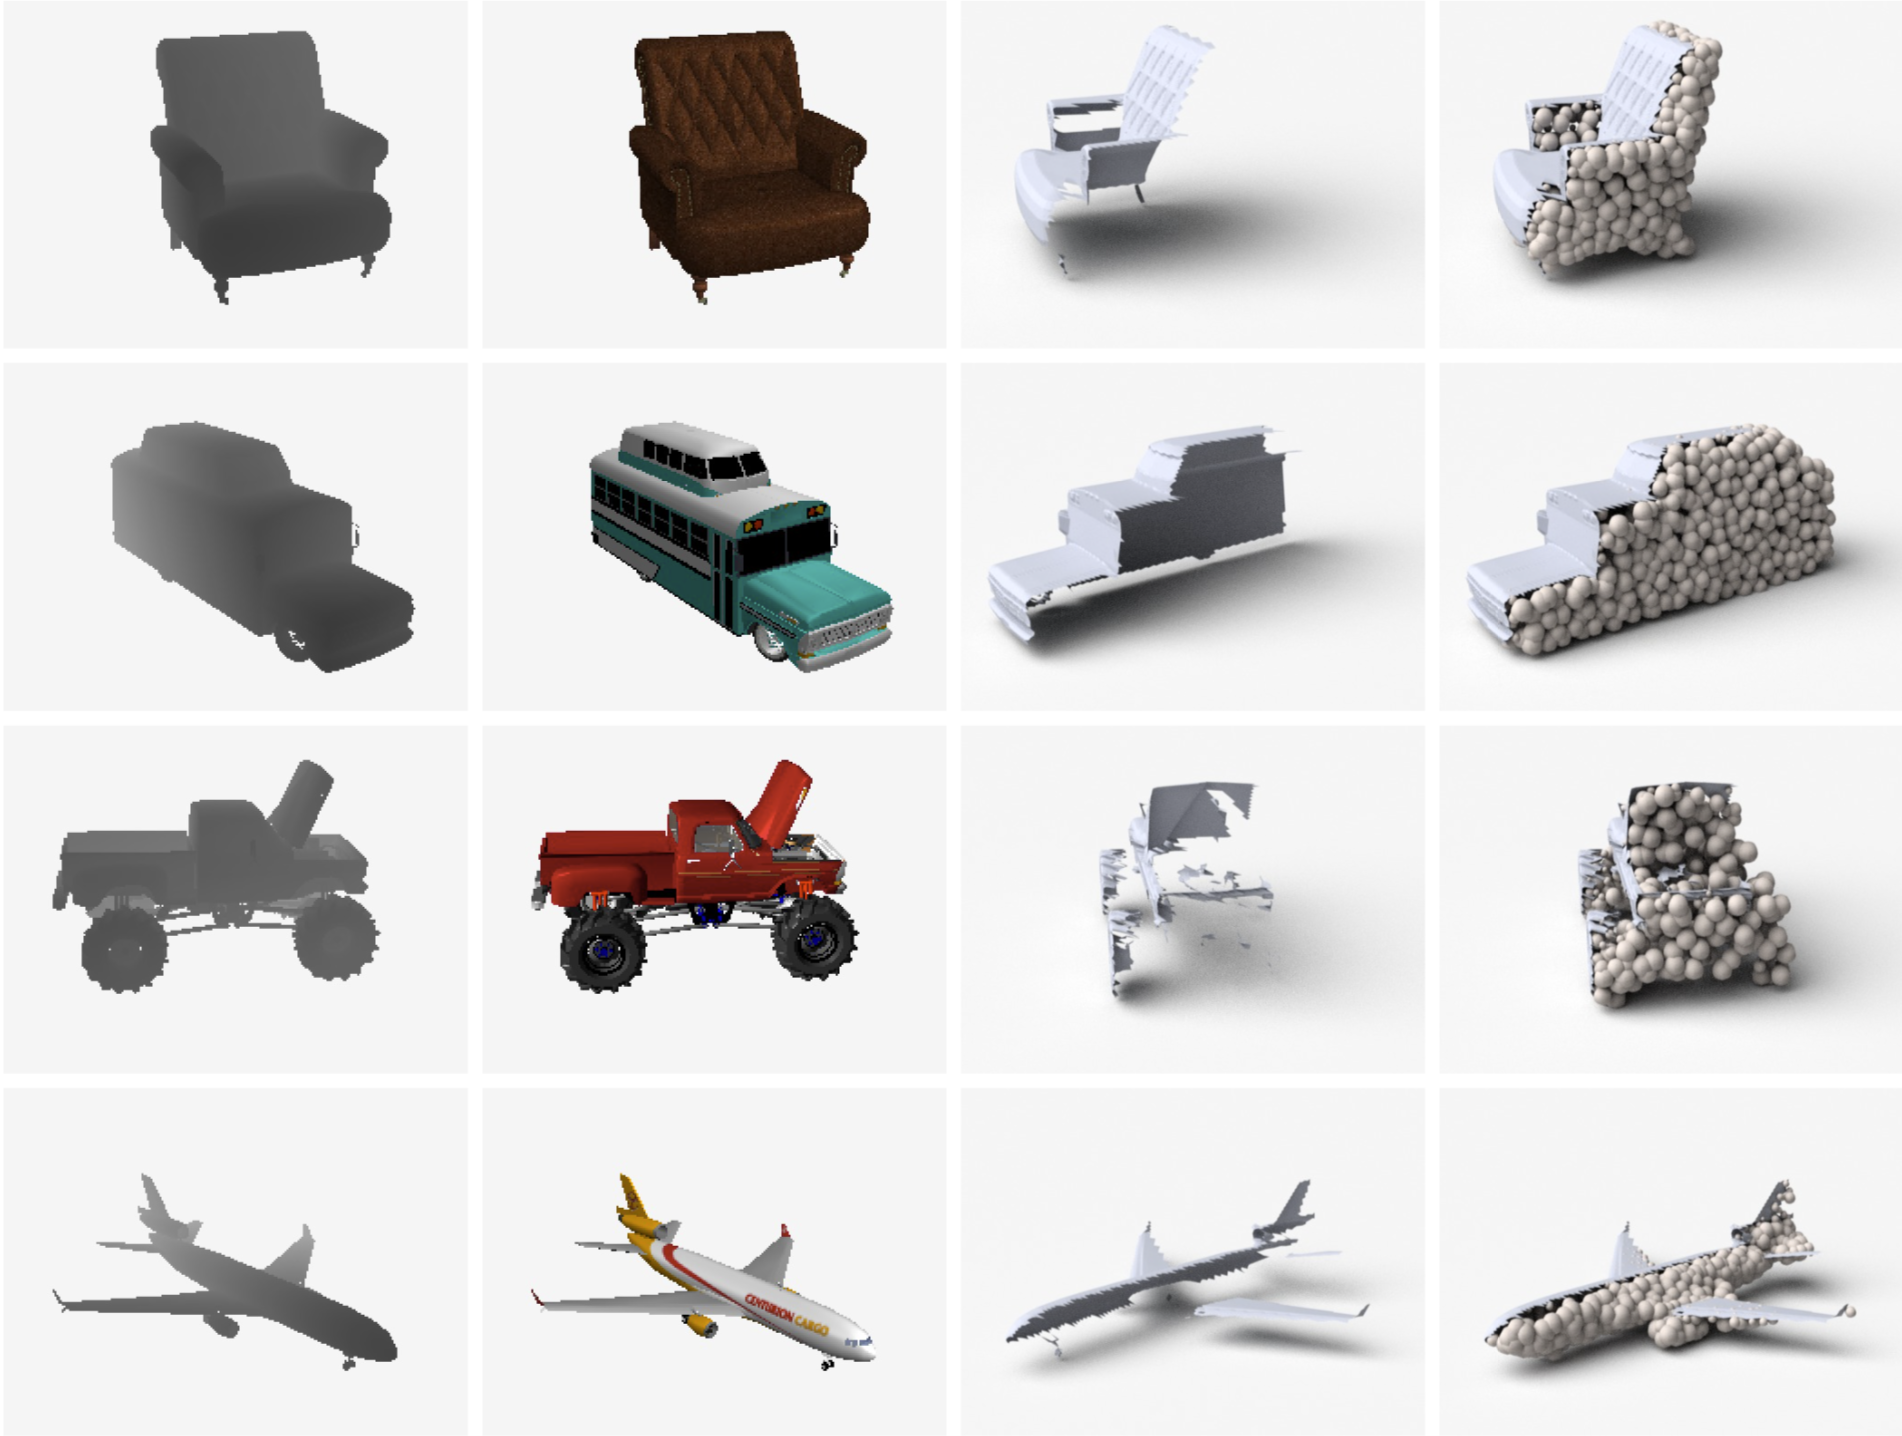
\includegraphics[width=.9\textwidth]{translate/complete}
	\caption[]{基于单视角 RGB-D 图像的形状补全}
	\label{fig:translate:complete}
\end{figure}

神经网络成功地猜测了模型的缺失部分。 % 通过使用
基于仓库中已有模型形状的先验知识,
系统可以利用对称(例如飞机两侧应该拥有相似且互为镜像的结构)和功能(例如拖拉机应该有圆柱状的轮子)等线索进行补全。
点云表示非常灵活,有助于解析三维物体的一般形状和拓扑关系。
我们可以进一步采取一些更细微的、直接利用局部几何结构的方法,对我们的结果进行后处理,以得到更加丰富的高频细节。





\subsection{预测多个合理的重建结果\label{section:translate:net_multi}}

在我们的网络中,随机变量 $r$ 可以使得网络在给定相同输入图像的情况下预测出多样的重建结果。
为了说明这一点,我们将 RGB 图像作为网络输入。 在训练期间,我们通过使用最小 $2$ 损失函数 (Min-of-2 loss, Mo2 loss)或 变分自编码器 处理随机性。
在真实情况未知的测试阶段,随机变量将从预先设定好的分布中进行采样。

\begin{figure}[h]
	\centering
	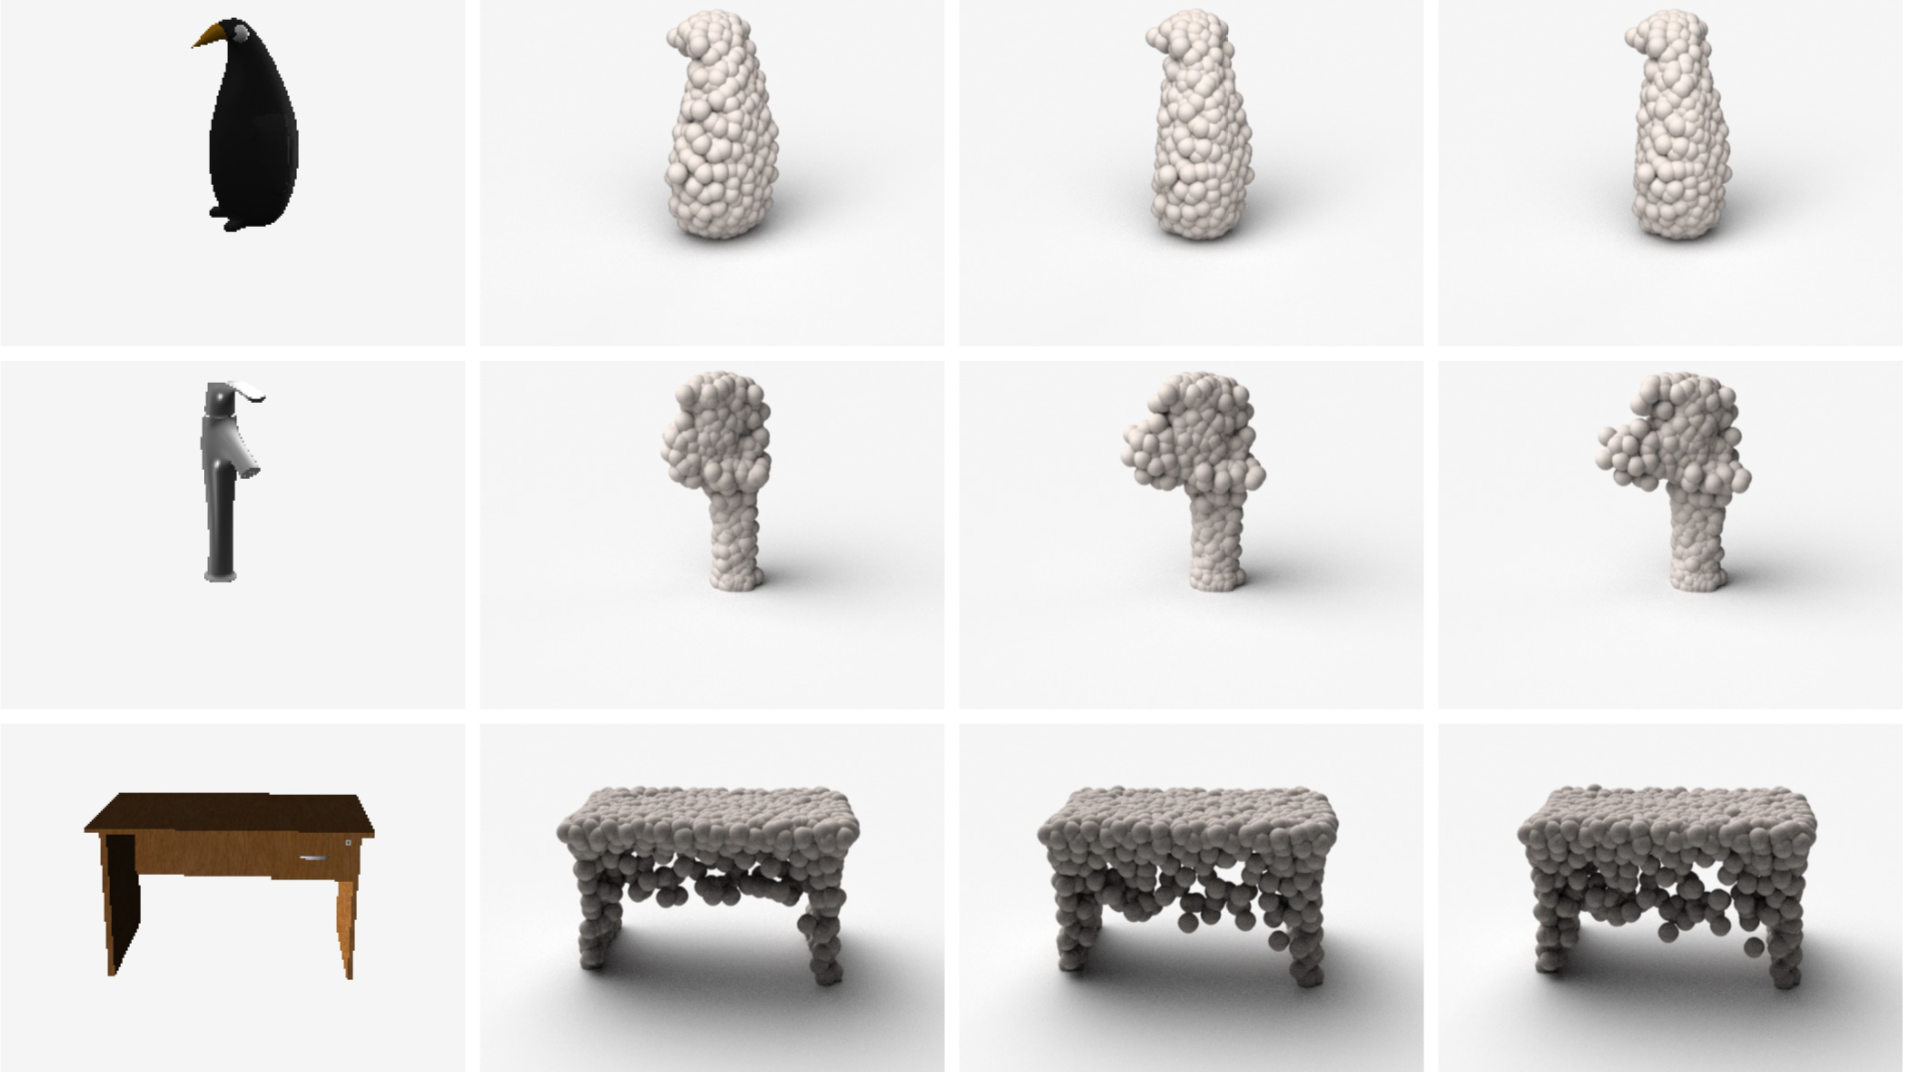
\includegraphics[width=.9\textwidth]{translate/rmon2}
	\caption[]{对单视角输入图像进行多次预测,并从不同的角度观察点云,以更好地显示差异。其中第一行的例子为半侧视图;第二行的例子为侧视图;最后一行的例子为后视图}
	\label{fig:translate:rmon2}
\end{figure}

\begin{figure}[h]
	\centering
	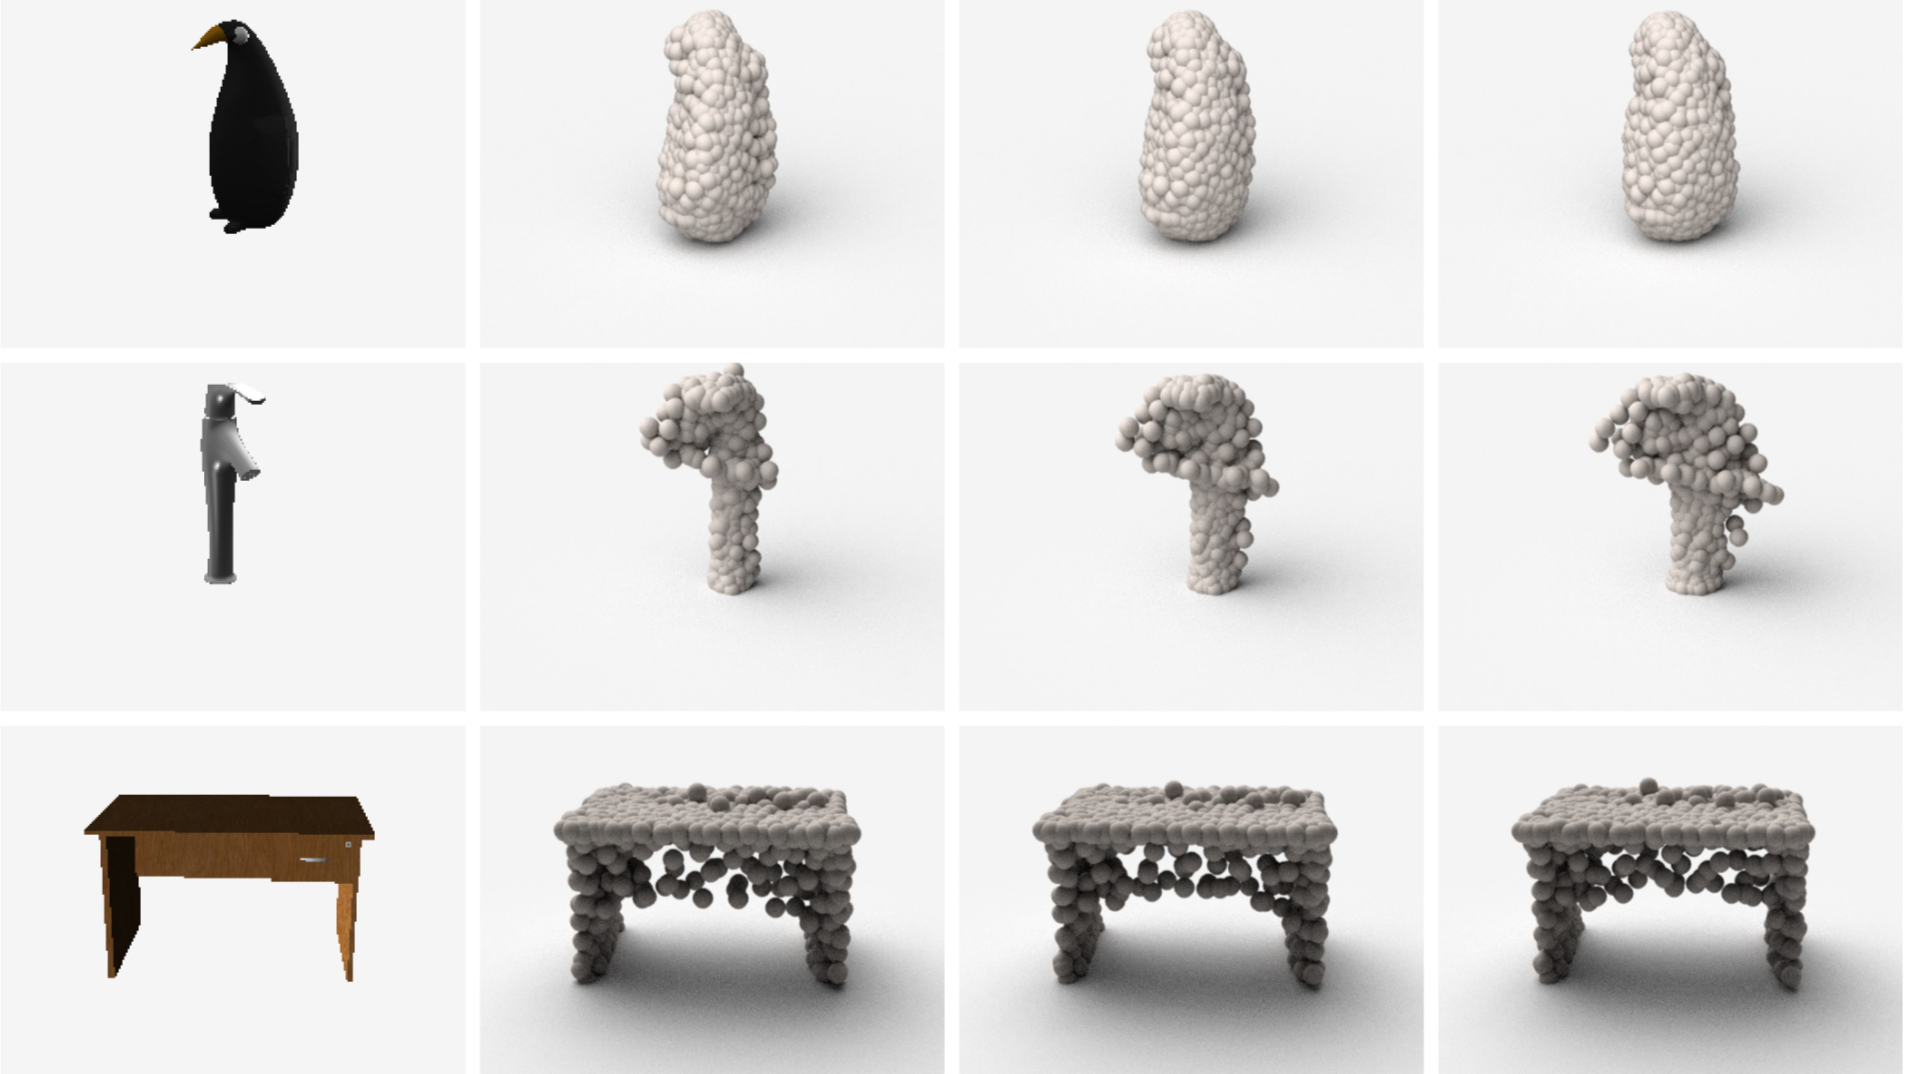
\includegraphics[width=.9\textwidth]{translate/rvae}
	\caption[]{通过变分自编码器训练的结果。其中第一行的例子为半侧视图;第二行的例子为侧视图;最后一行的例子为后视图}
	\label{fig:translate:rvae}
\end{figure}

图 \ref{fig:translate:rmon2} 绘制了使用本文算法得到的一组结果。
网络能够揭示输入图像中物体三维形状的不确定性。 对于神经网络已经非常确定的点,不同的预测之间位置移动非常小。
而在不确定性很大的点上(例如企鹅身体的厚度),其位置变化明显更大。 在此图中,我们用 最小 $2$ 损失函数 和 Chamfer 距离训练了我们的网络。
在图 \ref{fig:translate:rvae} 中,我们展示了使用 变分自编码器 训练的结果。 与最小 $2$ 损失函数的结果相比,变分自编码器的预测看起来更丰富;然而,它只捕捉了重建结果中局部的模糊性。


\subsection{网络设计分析 \label{section:translate:net_analyse}}

\begin{figure}[h]
	\centering
	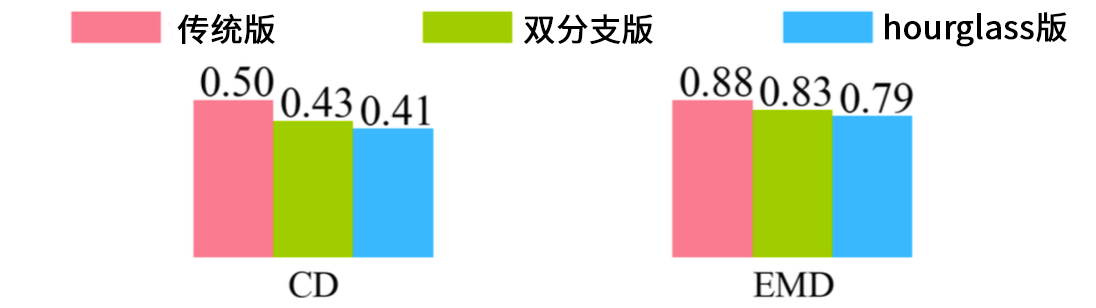
\includegraphics[width=.9\textwidth]{translate/cmpnet}
	\caption[]{通过 Chamfer 距离和推土机距离对不同的网络架构进行比较。 复杂的网络会带来稍好的结果}
	\label{fig:translate:cmpnet}
\end{figure}

{\heiti 将转置卷积分支和全连接分支结合对于重建结果的影响}
我们比较了不同的神经网络架构。
相对应的指标是基于我们自己渲染的训练数据计算得出的。
如图 \ref{fig:translate:cmpnet} 所示,引入转置卷积分支可显着提高性能。
在此基础上再加入一个 hourglass 结构也会提高性能。


\begin{figure}[h]
	\centering
	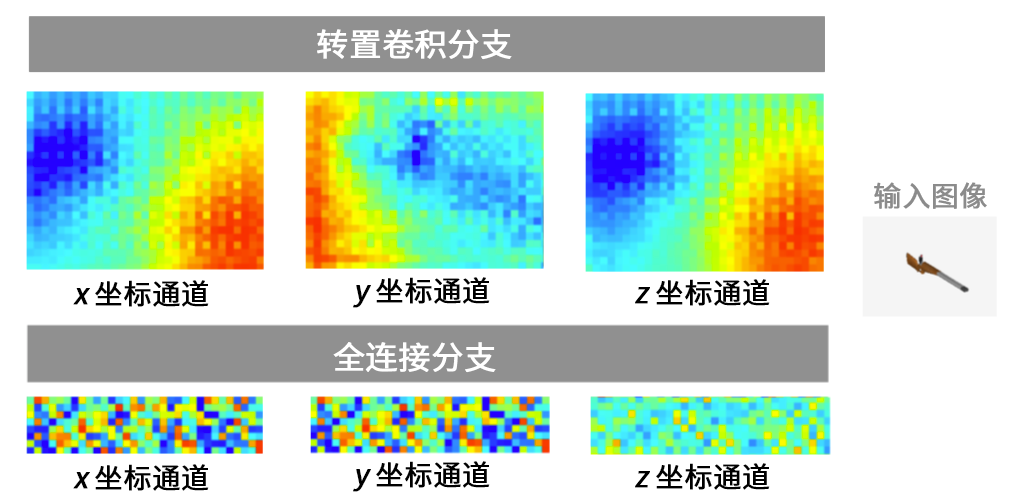
\includegraphics[width=.9\textwidth]{translate/vistb}
	\caption[]{ $x, y, z$ 坐标通道的可视化结果}
	\label{fig:translate:vistb}
\end{figure}


\begin{figure}[h]
	\centering
	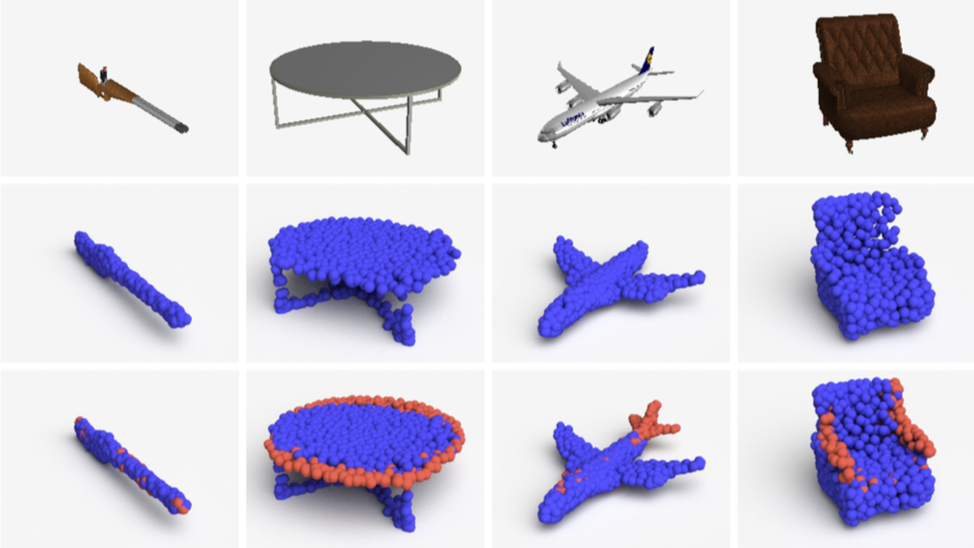
\includegraphics[width=.9\textwidth]{translate/vistb2}
	\caption[]{ 转置卷积分支和全连接分支预测结果的可视化。转置卷积分支的结果以蓝色表示,全连接分支的结果以红色表示}
	\label{fig:translate:vistb2}
\end{figure}

我们进一步将转置卷积分支和全连接分支的输出分开显示,
以更好地理解它们所完成的功能%的功能
。
在图 \ref{fig:translate:vistb} 中,重建结果中各点的坐标值 $x, y, z$ 被绘制成了三幅 二维 图像。 在转置卷积分支中,网络学会了如何使用卷积结构来构造一个围绕着物体表面折叠形成的二维曲面。在全连接的分支中,由于各通道未被有效排序,所以输出的结构较为混乱。%,组织性较差。

在图 \ref{fig:translate:vistb2} 中,我们渲染了着两个分支分别预测出的重建结果。
转置卷积分支通常擅长捕捉三维物体的“主体”,而全连接的分支
%完全连接的分支与更详细的组件
能够补充三维物体的细节,例如枪的尖端,飞机的尾部,沙发的两臂等。%形状互补。
这揭示了这两个分支的互补性。
% 预定义的
权重共享策略和节点连通性赋予了转置卷积分支更高的编码效率;%当两分支需要输出一致的三维结构时。
而全连接的分支往往更加灵活,但每个点的独立性却消耗着更多的网络容量。


\begin{figure}[h]
	\centering
	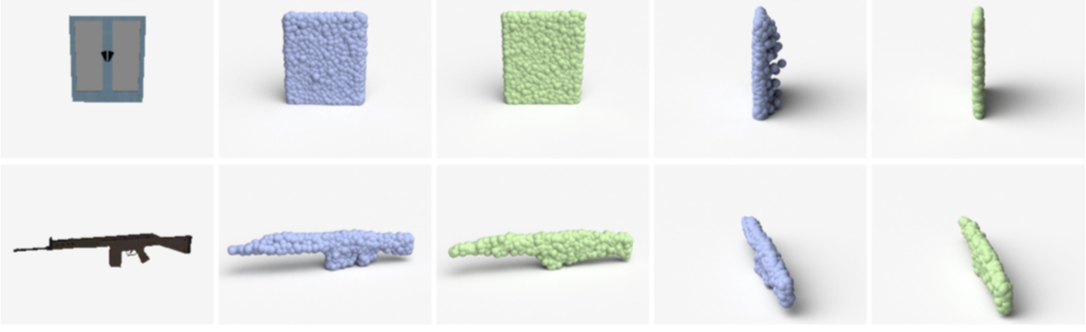
\includegraphics[width=.9\textwidth]{translate/cmpdis}
	\caption[]{
		网络分别由 Chamfer 距离和推土机距离训练后,所得重建结果的差异。左方的蓝色点云是由 Chamfer 距离训练得出的,右方的绿色点云是由推土机距离训练得出的}
	\label{fig:translate:cmpdis}
\end{figure}

{\heiti 距离度量的分析}
损失函数的%不同
选择对网络的重建结果%预测模式
有明显的影响。
图 \ref{fig:translate:cmpdis} 表明了由 Chamfer 距离和推土机距离进行相应的训练后,两个网络之间的差异。
由 Chamfer 距离训练的网络倾向于在其不确定的区域(例如门后)散射几个点,
但能够更好地保持门握把的具体形状。
相比之下,由推土机距离%EMD培训
训练的网络
可以
产生更紧凑的结果,但有时会过度缩小局部结构。
这与前面在合成数据上的实验结果是一致的。


\begin{figure}[h]
	\centering
	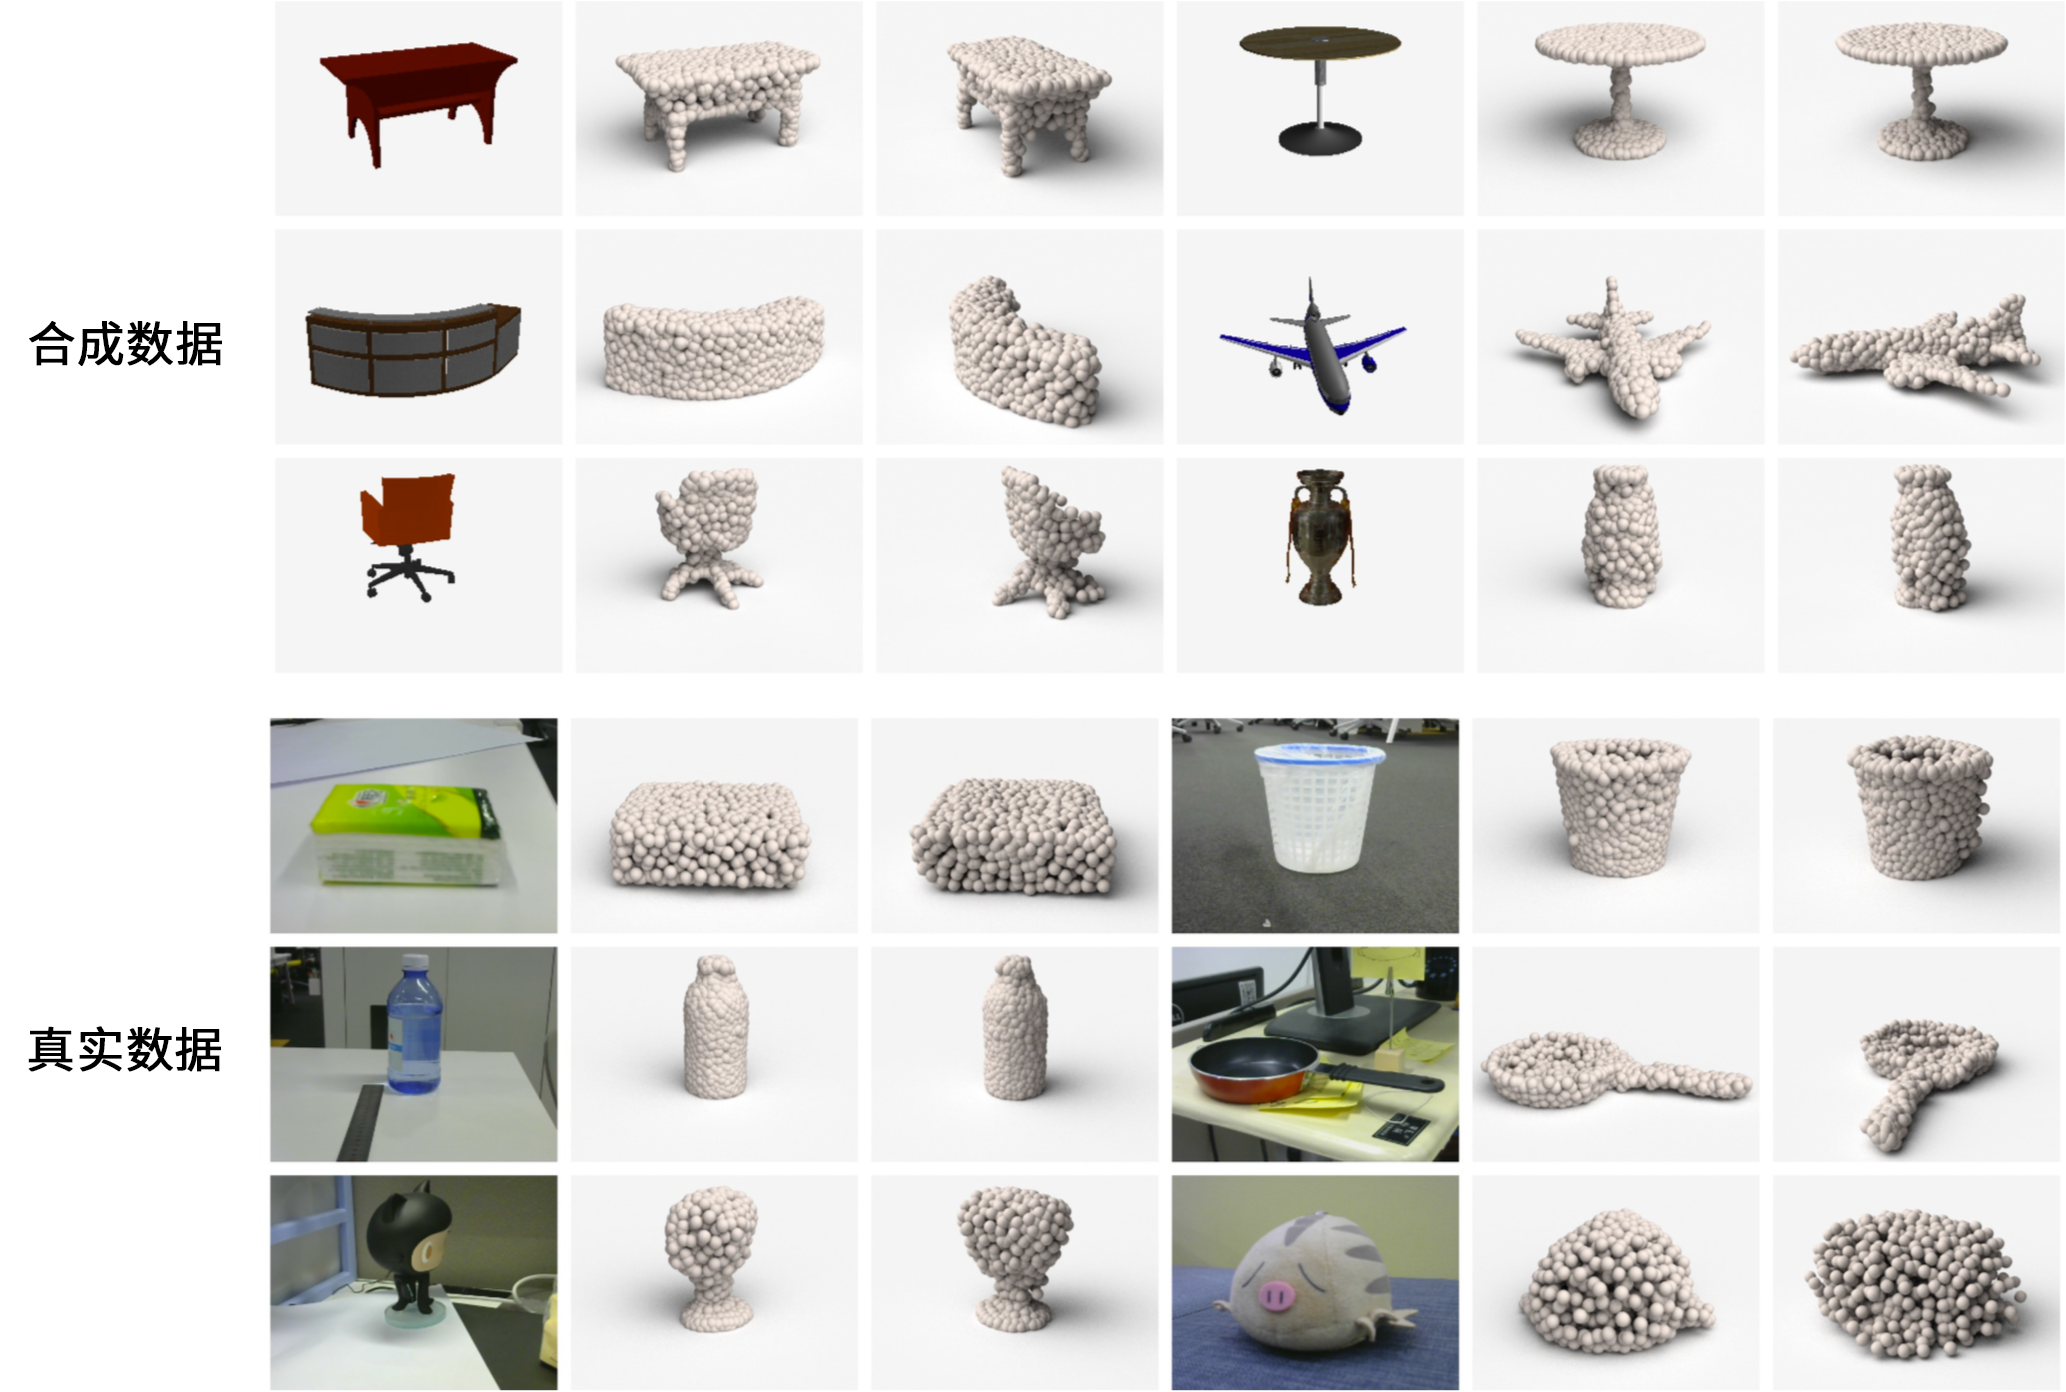
\includegraphics[width=.9\textwidth]{translate/realres}
	\caption[]{
		在合成图像和真实图像上的重建结果}
	\label{fig:translate:realres}
\end{figure}

\subsection{在现实世界中的真实图像上的更多结果和应用}

图 \ref{fig:translate:realres} 列出了关于合成数据和真实图像的更多重建示例。 对于真实世界的照片,我们提供了 mask,以掩盖背景,同时指示出待重建的对象。 我们的算法虽然仅通过合成数据进行训练,但仍然可以在真实图像上取得很好的结果。
我们在本文最后的图 \ref{fig:translate:val5} 中绘制了我们验证集的前 5 个小批次(共 160 个案例)的重建结果。
我们并列展示了通过 Chamfer 距离和推土机距离训练的网络的重建结果差异。 由于 ShapeNet 数据集的多样性,我们的系统能够处理多种类型的三维物体。

\begin{figure}[h]
	\centering
	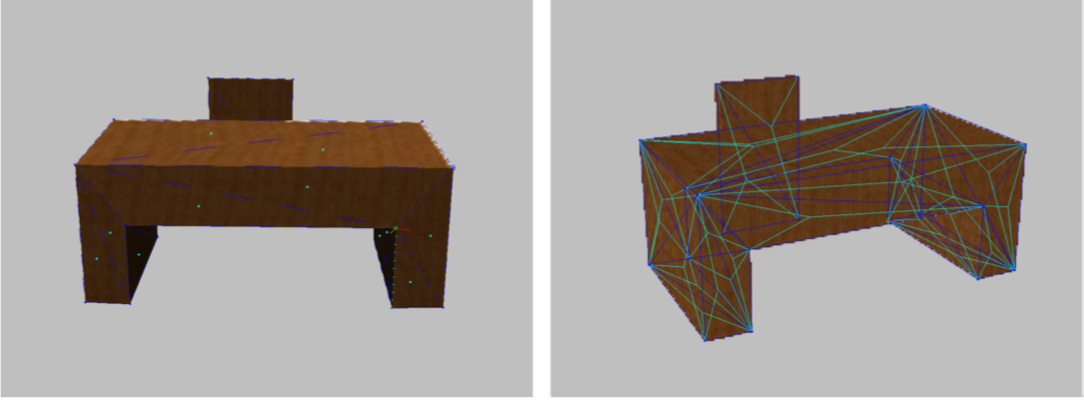
\includegraphics[width=.9\textwidth]{translate/gui}
	\caption[]{用于手动建模的图形用户界面工具。 用户可以在三维视图中更改视点,编辑顶点位置和连通性。 我们同时还提供输入图像的显示,以便于将二维图像和三维重建结果对齐。}
	\label{fig:translate:gui}
\end{figure}

\subsection{关于人类基于单视角图像三维重建能力的分析}
我们进行了人类三维重建能力的研究,
%以提供我们在渲染数据集上报告的当前CD和EMD值的参考。
作为本文算法在我们渲染的数据集上各项指标的参考。
我们为被测试人提供了一个具有图形用户界面的工具,如图 \ref{fig:translate:gui} 所示,用于从图像中创建三角面片。
该工具使用户能够编辑三角面片,并将建模对象对准输入的图像。 被测试人从我们验证集的输入图像中总共创建了 16 个模型。
我们进一步从这些模型中采样得到 $N = \numprint{1024}$ 个点。

\begin{figure}[h]
	\centering
	\subcaptionbox{\label{fig:translate:humanemd}}
	{
		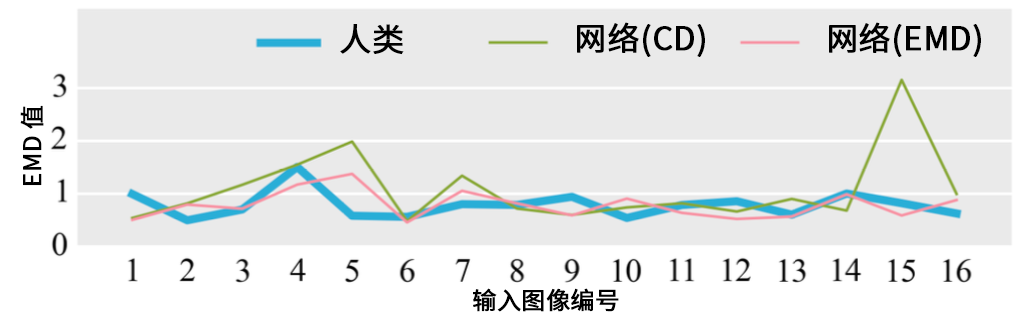
\includegraphics[width=.8\textwidth]{translate/humanemd}
	}
	\subcaptionbox{\label{fig:translate:humancd}}
	{
		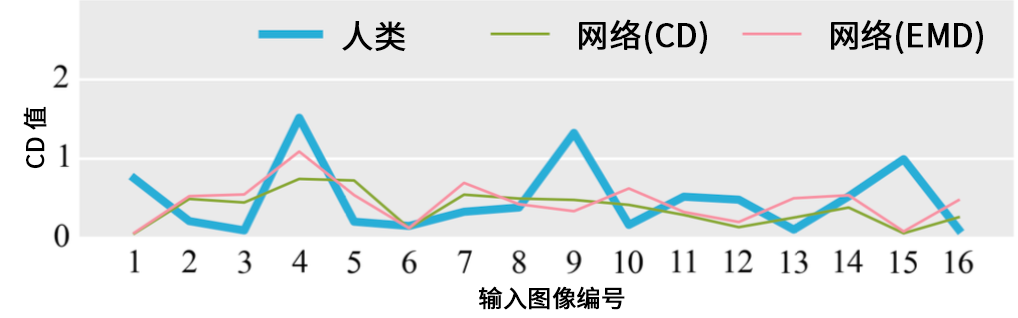
\includegraphics[width=.8\textwidth]{translate/humancd}
	}
	\subcaptionbox{\label{fig:translate:humaneg}}
	{
		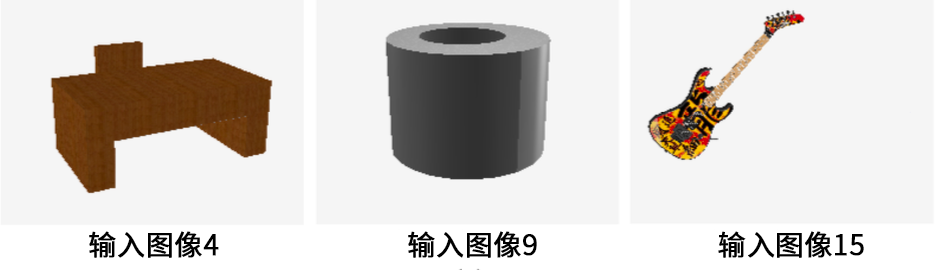
\includegraphics[width=.6\textwidth]{translate/humaneg}
	}
	\caption[]{被测试人提供的重建结果、使用 Chamfer 距离训练所得神经网络的重建结果以及使用 推土机 距离训练所得神经网络的重建结果,三者在测试集上的对比。
		\subref{fig:translate:humanemd} 比较推土机距离;
		\subref{fig:translate:humancd} 比较 Chamfer 距离;
		\subref{fig:translate:humaneg} 编号为 4、9 和 19 的图像。人类对此图的重建表现不佳}
	\label{fig:translate:human}
\end{figure}

如图 \ref{fig:translate:human} 所示,在大多数情况下,通过神经网络
得到的重建结果
%重构的EMD和CD值都
与人工手动重建的结果,在 Chamfer 距离和推土机距离两项指标下旗鼓相当。
我们观察到,人工重建的三维模型主要凭借重力(例如椅子腿应接触地面)和对称性来推断物体的形状和位置。当物体被部分遮挡(例如被桌子所遮挡的椅子)、有歧义(不清楚罐子是否有底部)或几何线索的显示不充分时(例如吉他具有非多边形的形状,且并且不接触地面),如编号为 4 、 9 和 15 的输入图像所示,人工重建的结果很差。
使用推土机距离训练的神经网络在两个指标下表现相当好。
然而,因为 Chamfer 距离只强调最佳匹配点,所以使用 Chamfer 距离训练的网络并不总是产生均匀密度的预测,并且在某些情况下
%会遭受高EMD值
推土机距离的指标会非常不理想
。

\begin{figure}[h]
	\centering
	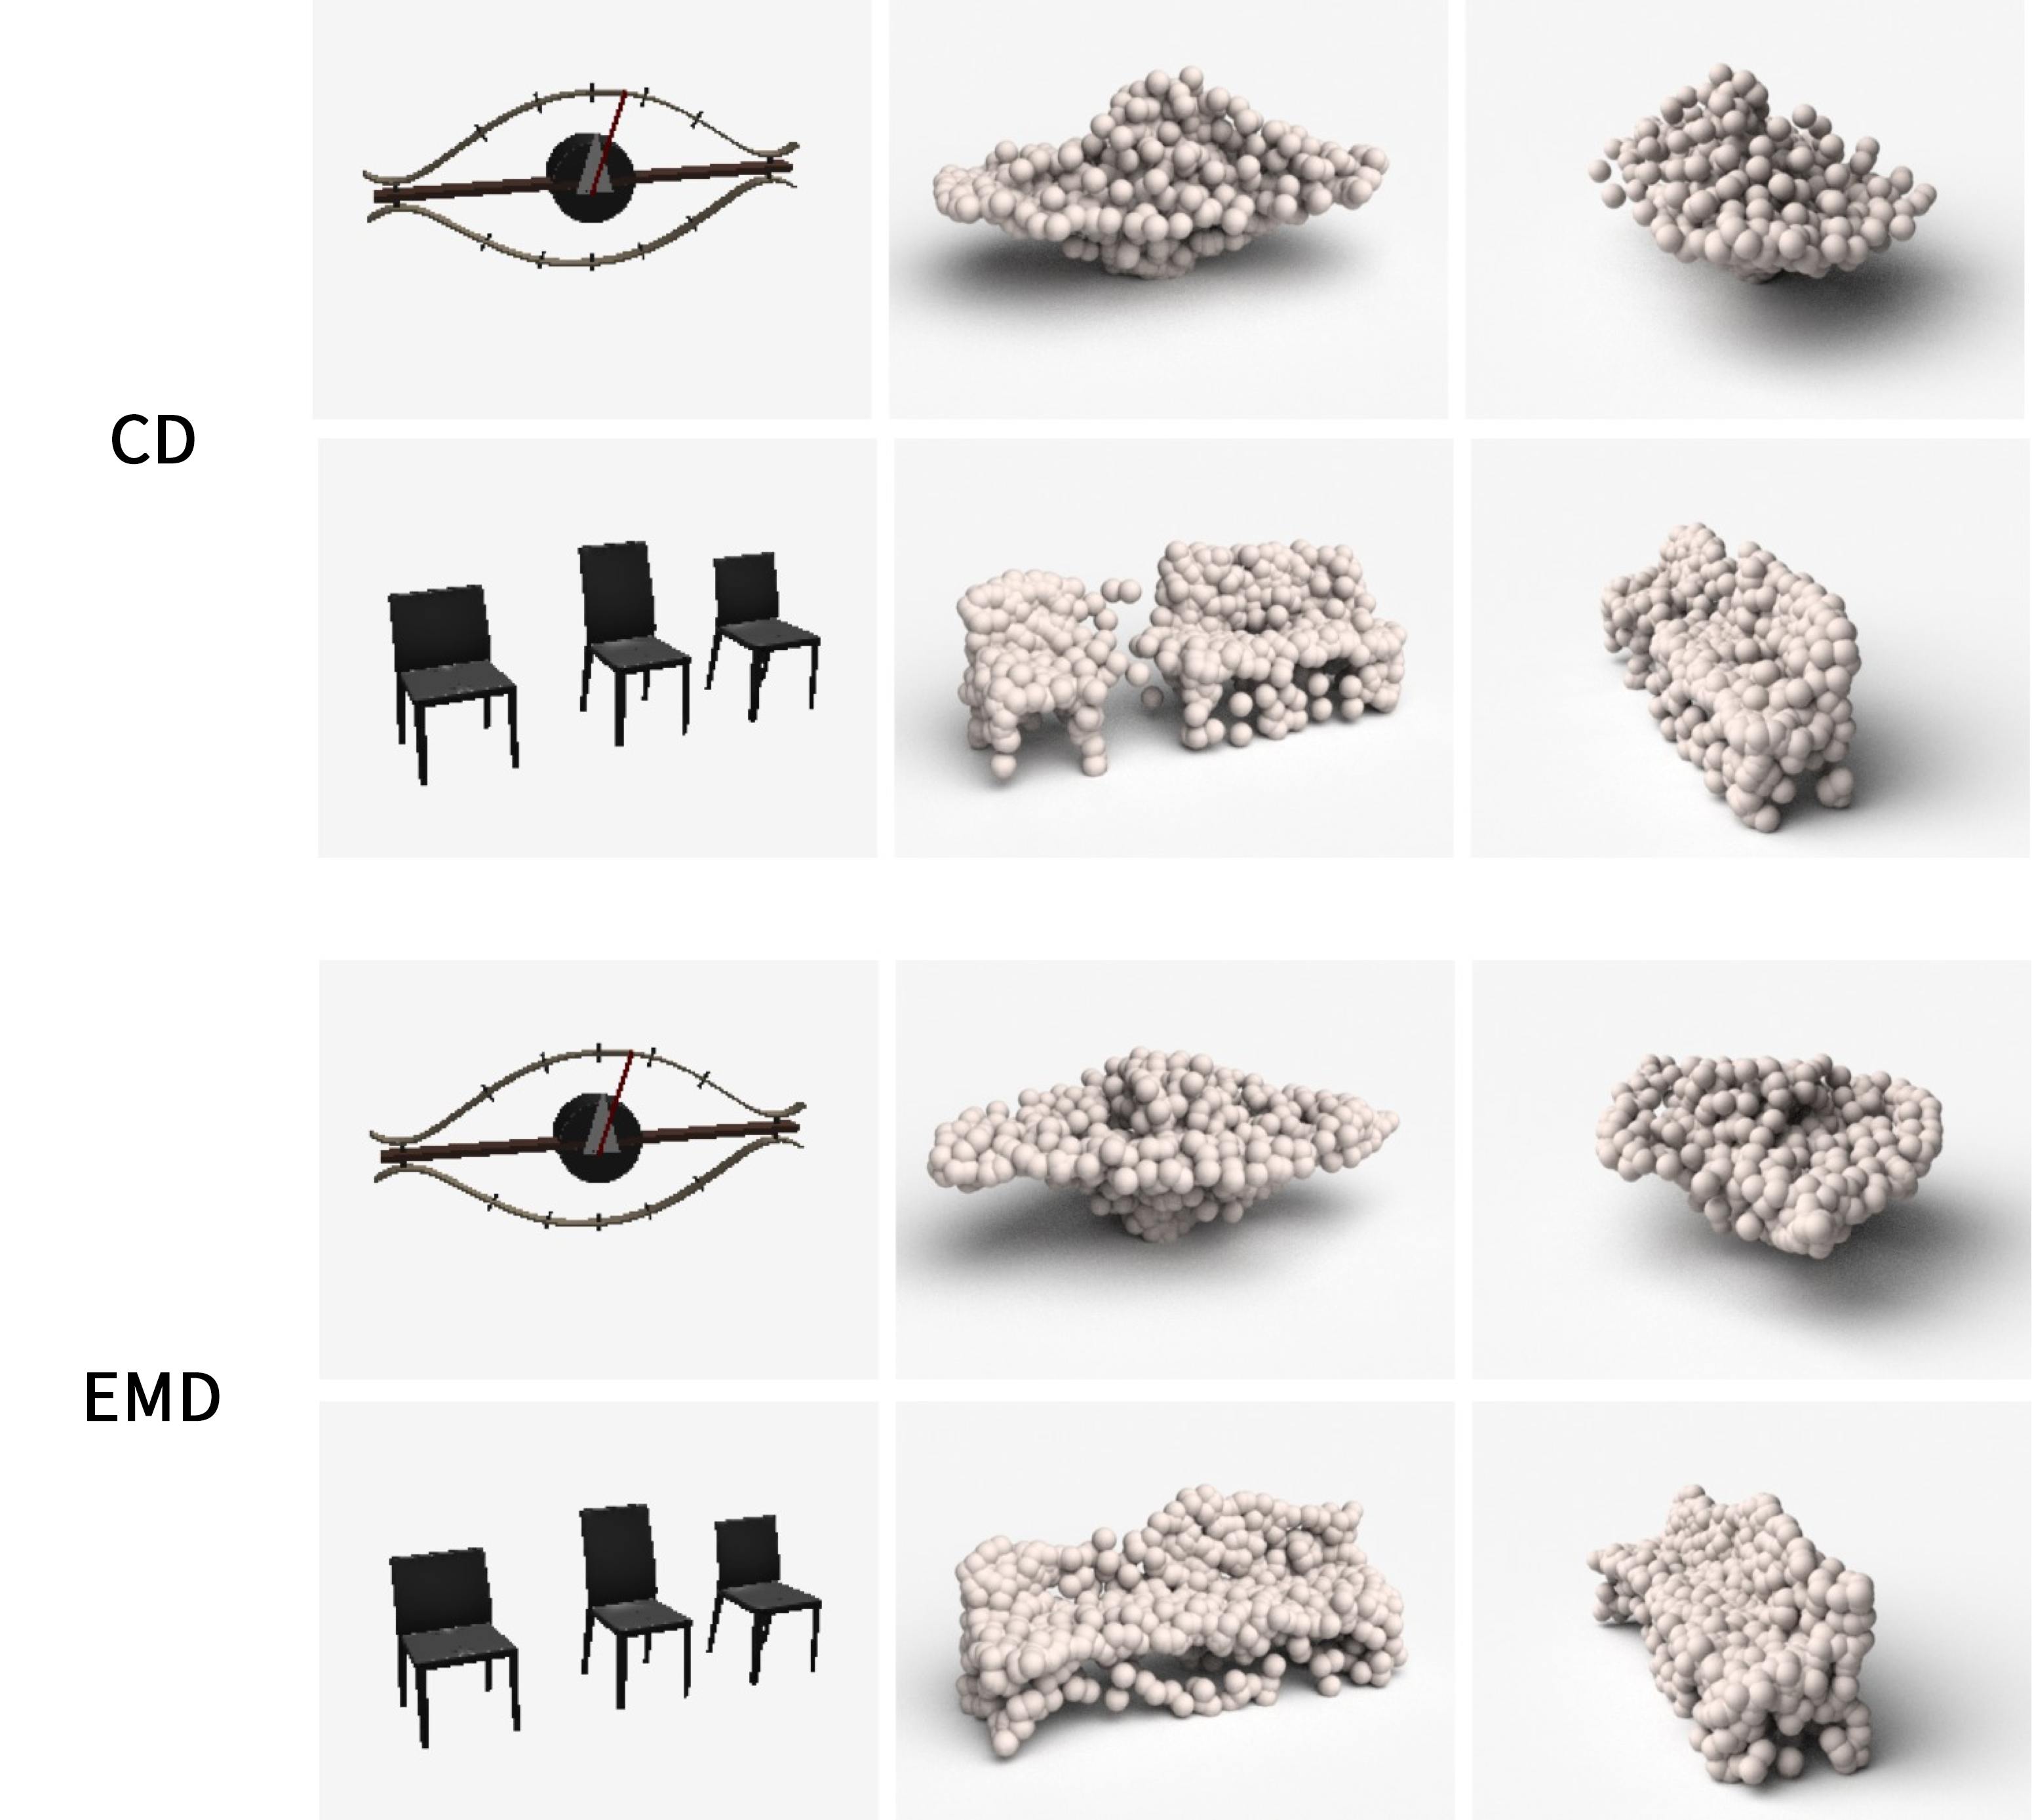
\includegraphics[width=.6\textwidth]{translate/fail}
	\caption[]{本方法在验证集上的失败案例。
		上半部分是由 Chamfer 距离训练所得神经网络的重建结果;
		下半部分是由推土机距离训练所得神经网络的重建结果。
		两个网络的重建结果都不令人满意。
	}
	\label{fig:translate:fail}
\end{figure}

\subsection{失败案例分析}
我们在本工作渲染出的验证集上,展示了本方法无法有效处理的代表性失败案例。
这些失败案例有两种情况,我们对于每种情况都通过图 \ref{fig:translate:fail} 中的一个输入案例来加以说明。
在第一种失败案例中,%神经网络重建出一种完全无法被理解的物体形状。 那么
神经网络完全不清楚待重建物体的具体形状,
因此网络试图用类似的东西来解释输入,例如没有翅膀的飞机。但这%根本没有任何意义,
完全是不正确的。%从原理上说是错误的。
在第二种失败案例中,神经网络看到了多个对象的组合而成的输入图像。 由于我们尚未实施任何检测或关注机制,因此网络会产生扭曲的输出。



\subsection{实现细节 \label{section:translate:psg_detail}}


{\heiti 网络参数和训练过程}
我们的网络适用于 $192 \times 256$ 的输入图像。
转置卷积分支产生 $768$ 点,对应于 $32 \times 24$ 的 三通道图像。 完全连接的分支产生剩余的 $256$ 个点。
卷积层在最大分辨率中具有16个不同得特征通道,并且在每次分辨率减半后,通道数量会增加一倍。
我们使用跨步卷积 (Strided Convolution) 而非最大池化 (Max Pooling)来提高计算速度。 训练过程通过 TensorFlow 实现。
我们的训练过程包括了 300000 步梯度下降,每一步都使用大小为 32 的小批次 (Mini-batch) 计算。我们采取了 Adam 作为我们的优化器。
我们观察到:即使没有使用批标准化 (Batch Normalization) 策略,训练过程也非常顺利。网络中的所有激活函数都是线性整流函数。

{\heiti 后处理过程}
我们使用一个局部化的方法来将点云处理后处理为体积表示。
首先,我们使用双线性插值将点云嵌入到 $32 \times 32 \times 32$ 的网格中。
该过程可以理解为:将点视为 $1 \times 1 \times 1$ 大小的立方体,并且计算每个网格单元的与其交集的体积平均值,即体积占用表示。最后,每个体素点会再次检查周围的体素,以确定最终的值。
%我们将它作为一个训练过的具有6层3x3x3卷积的三维卷积神经网络来实现。
我们通过训练一个有 6 层卷积核大小为 $3 \times 3 \times 3$  的三维卷积神经网络,实现了上述转换过程。
此后处理网络通过将交并比作为损失函数,与点云生成网络 %相同的训练分区上进行
一起进行训练。
为了补偿不同体积的物体之间的点密度差异,我们训练了另一个网络来预测物体的体积。
预测出的体积值,也将会作为三维卷积神经网络的输入,与已有的体积占用表示共同计算出最终的体素表示结果。
% 使用由EMD或CD训练的点云生成网络足以胜过\threedrsns的结果。
无论是使用 Chamfer 距离还是使用推土机距离训练,得到的点云生成网络都足以胜过 \threedrsns 的结果。
%主要论文中报告的最大性能是通过将网络的预测馈送到后处理网络中获得的。
本文中记载的重建结果指标是通过将网络的预测结果经过后处理网络转换后,才计算得出的。
此外,我们还注意到:体素预测网络并不一定要超越 \threedrsns。然而,它%始终如一地提高性能,所以
仍然能够给出优于 \threedrsns 的提升,因此我们在实验中保留了
%这个组件
该体素预测网络
。

\begin{figure}[!hp]
	\centering
	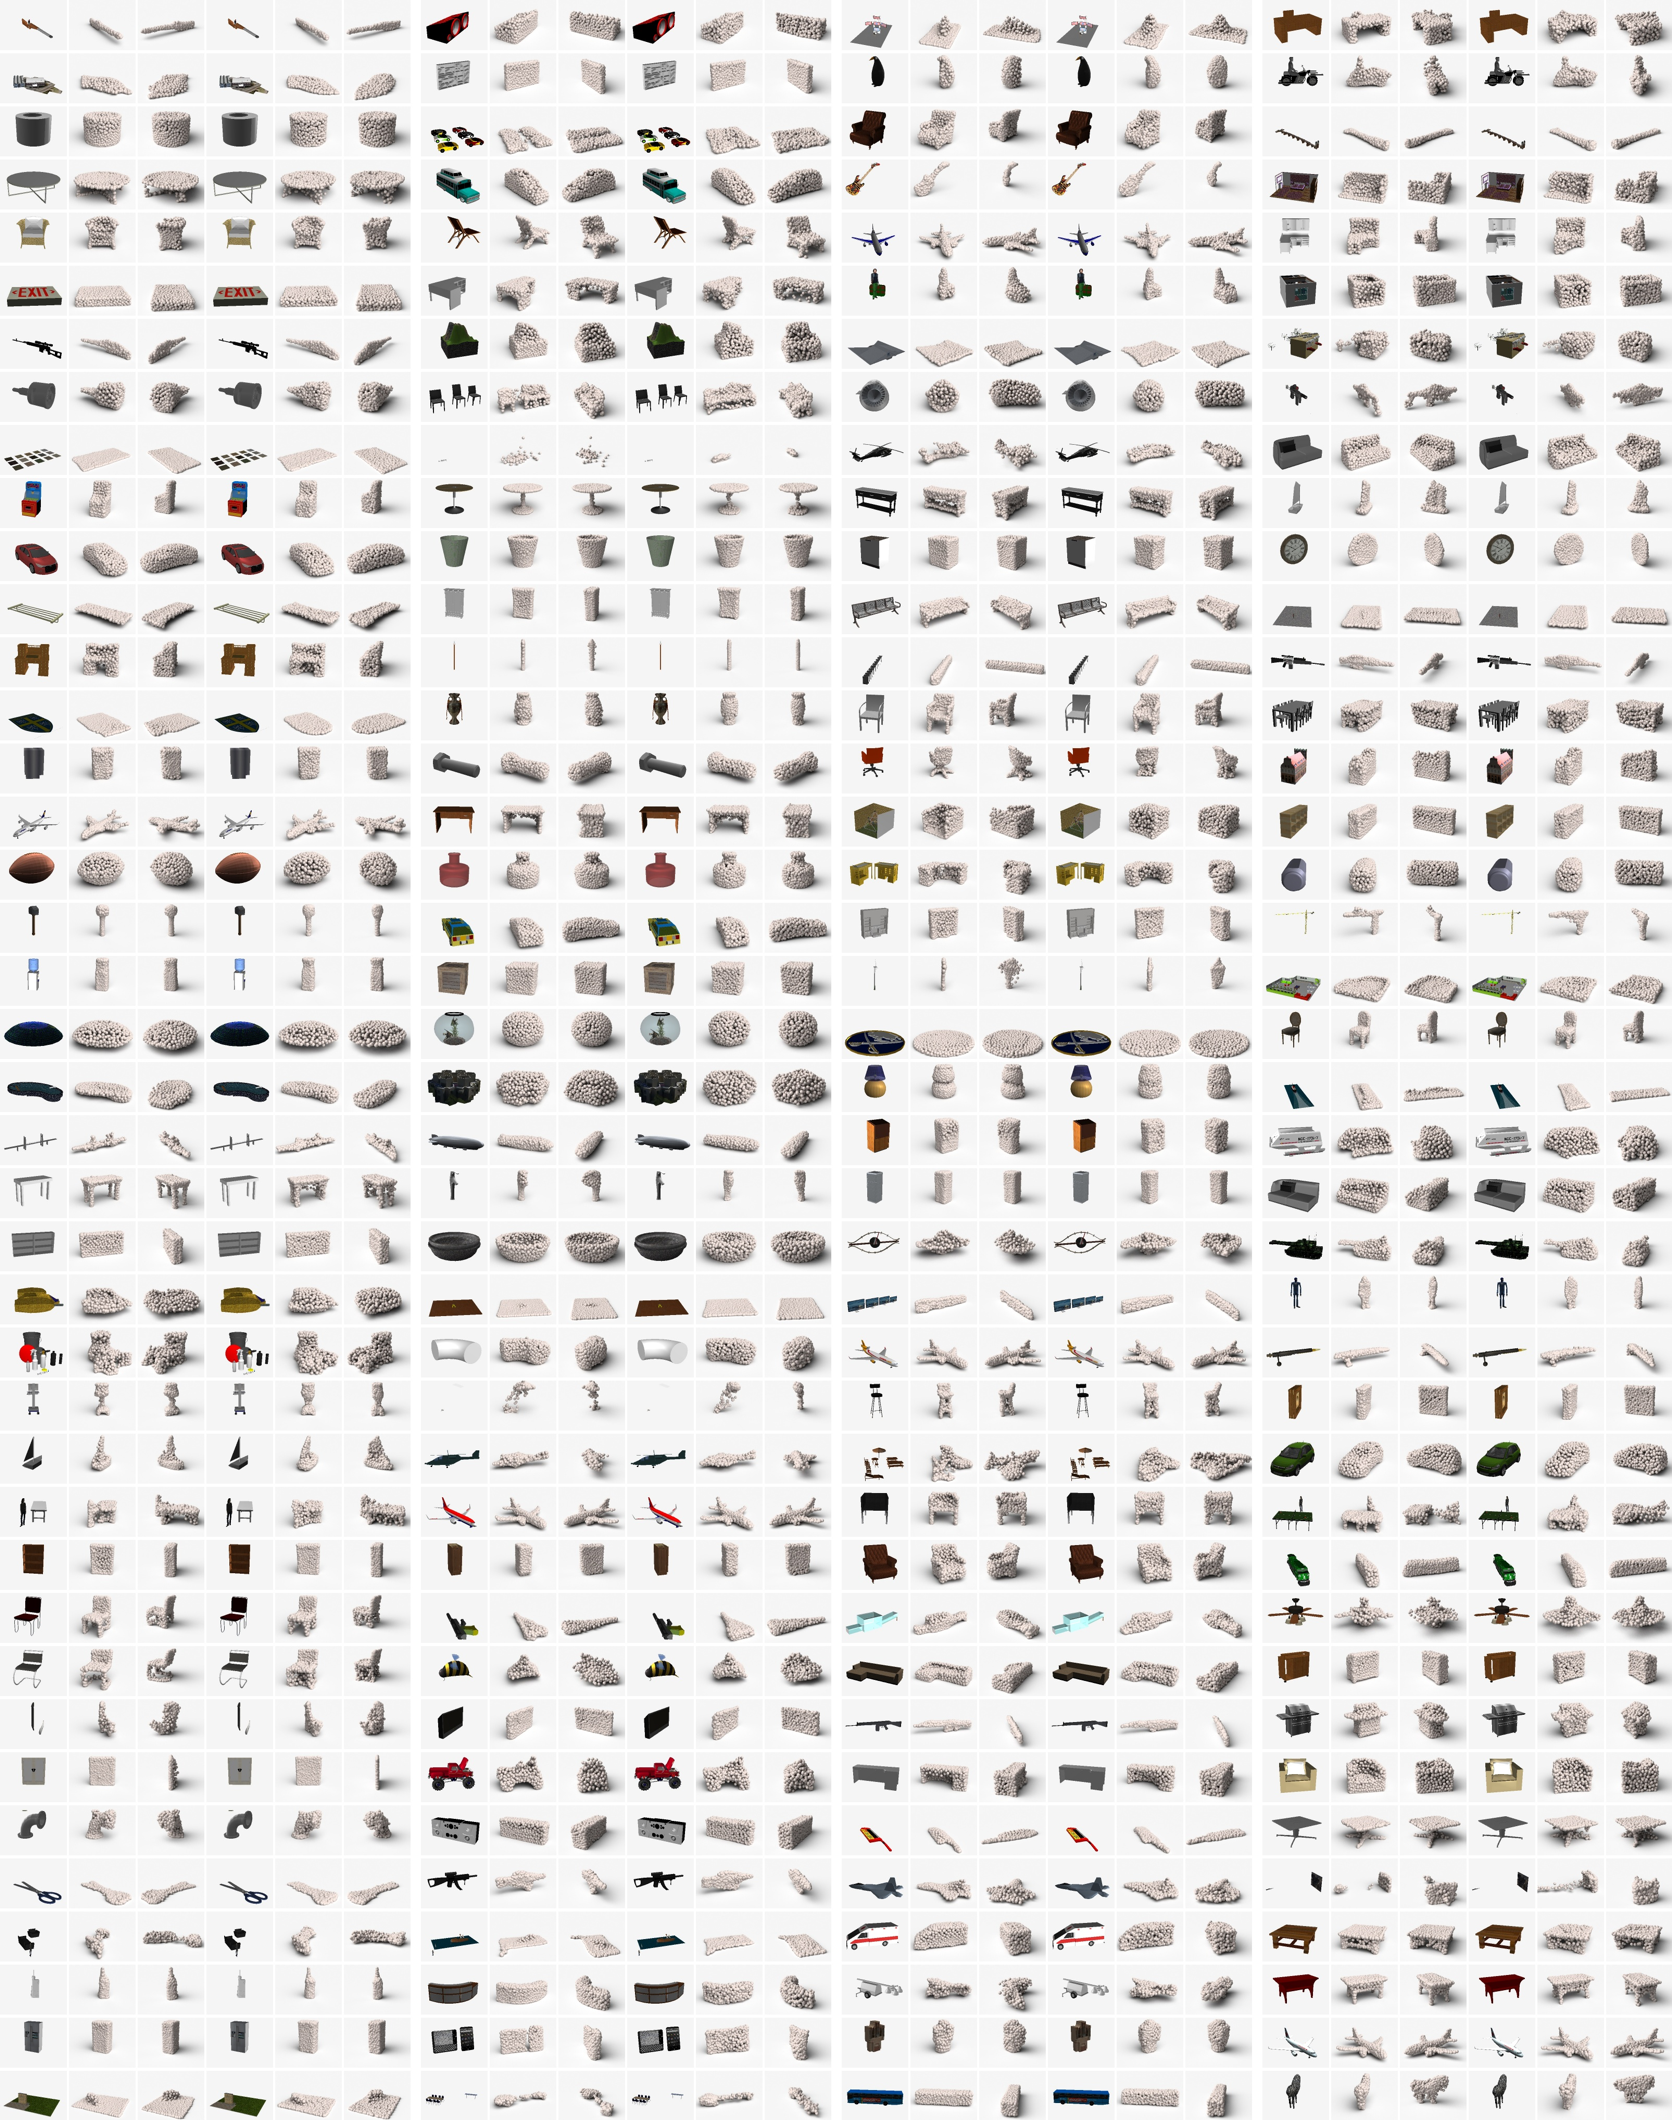
\includegraphics[width=.999\textwidth]{translate/val5}
	\caption[]{ 验证集的前 5 个小批次的重建结果。
		通过 Chamfer 距离训练得出的重建结果在左侧;而通过推土机距离训练得出的重建结果在右侧}
	\label{fig:translate:val5}
\end{figure}

\section{讨论}
虽然本文解决了一个实际应用问题——三维重建,但我们仍然触及了两个基本的理论问题:
第一,如何生成一组无序的实体。为了构建%更
复杂
%组合
数据结构的生成模型,例如图 (Graph) 等,学习如何生成一个集合可能是一个很好的起点。 其次,如何在回归问题中捕捉到真实情况的不确定性。 除了三维重建之外,许多回归问题都可能具有这种固有的不确定性。 我们通过对已有的损失函数进行包装,以构建最小 $n$ 损失的解决方案,可以推广到这些问题之上。


\begin{center}
	\section*{{\songti \xiaosi 书面翻译对应的原文索引}}
\end{center}

\begin{translationbib}
	% [1] 
	\item J. Aloimonos. Shape from texture. Biological cybernetics, 58(5):345–360, 1988.
	% [2] 
	\item D.P.Bertsekas.Adistributedasynchronousrelaxation algorithm for the assignment problem. In Decision and Control, 1985 24th IEEE Conference on, pages 1703–1704. IEEE, 1985.
	% [3] 
	\item J. Carreira, S. Vicente, L. Agapito, and J. Batista. Lifting object detection datasets into 3d. IEEE Trans- actions on Pattern Analysis and Machine Intelligence, 38(7):1342–1355, 2016.
	% [4] 
	\item A. X. Chang, T. Funkhouser, L. Guibas, P. Hanrahan, Q. Huang, Z. Li, S. Savarese, M. Savva, S. Song, H. Su, J. Xiao, L. Yi, and F. Yu. ShapeNet: An Information-Rich 3D Model Repository. Technical Report arXiv:1512.03012 [cs.GR], 2015.
	% [5] 
	\item C.B.Choy,D.Xu,J.Gwak,K.Chen,andS.Savarese. 3d-r2n2: A unified approach for single and multi- view 3d object reconstruction. arXiv preprint arXiv:1604.00449, 2016.
	% [6] 
	\item C. Doersch. Tutorial on variational autoencoders. arXiv preprint arXiv:1606.05908, 2016.
	% [7] 
	\item D. Eigen, C. Puhrsch, and R. Fergus. Depth map prediction from a single image using a multi-scale deep network. In Advances in neural information processing systems, pages 2366–2374, 2014.
	% [8] 
	\item Y. Eldar, M. Lindenbaum, M. Porat, and Y. Y. Zeevi. The farthest point strategy for progressive image sampling. IEEE Transactions on Image Processing, 6(9):1305–1315, 1997.
	% [9] 
	\item D. F. Fouhey, A. Gupta, and M. Hebert. Data-driven 3D primitives for single image understanding. In ICCV, 2013.
	% [10] 
	\item J. Fuentes-Pacheco, J. Ruiz-Ascencio, and J. M. Rendo ́n-Mancha. Visual simultaneous localization and mapping: a survey. Artificial Intelligence Review, 43(1):55–81, 2015.
	% [11] 
	\item K. H{\"a}ming and G. Peters. The structure-from-motion reconstruction pipeline–a survey with focus on short image sequences. Kybernetika, 46(5):926–937, 2010.
	% [12] 
	\item D. Hoiem, A. A. Efros, and M. Hebert. Automatic photo pop-up. ACM transactions on graphics (TOG), 24(3):577–584, 2005.
	% [13] 
	\item B. K. Horn. Obtaining shape from shading informa- tion. In Shape from shading, pages 123–171. MIT press, 1989.
	% [14] 
	\item Q. Huang, H. Wang, and V. Koltun. Single-view reconstruction via joint analysis of image and shape collections. ACM Transactions on Graphics (TOG), 34(4):87, 2015.
	% [15] 
	\item A. Kar, S. Tulsiani, J. Carreira, and J. Malik. Category-specific object reconstruction from a single image. In CVPR, 2015.
	% [16] 
	\item D. Maturana and S. Scherer. Voxnet: A 3d convolu- tional neural network for real-time object recognition. In IEEE/RSJ International Conference on Intelligent Robots and Systems, September 2015.
	% [17] 
	\item M. Mirza and S. Osindero. Conditional generative adversarial nets. arXiv preprint arXiv:1411.1784, 2014.
	% [18] 
	\item A. Newell, K. Yang, and J. Deng. Stacked hourglass networks for human pose estimation. arXiv preprint arXiv:1603.06937, 2016.
	% [19] 
	\item D. J. Rezende, S. Eslami, S. Mohamed, P. Battaglia, M. Jaderberg, and N. Heess. Unsupervised learn- ing of 3d structure from images. arXiv preprint arXiv:1607.00662, 2016.
	% [20] 
	\item Y. Rubner, C. Tomasi, and L. J. Guibas. The earth mover’s distance as a metric for image retrieval. International journal of computer vision, 40(2):99– 121, 2000.
	% [21] 
	\item A. Saxena, M. Sun, and A. Y. Ng. Make3d: Learning 3d scene structure from a single still image. IEEE transactions on pattern analysis and machine intelligence, 31(5):824–840, 2009.
	% [22] 
	\item H. Su, Q. Huang, N. J. Mitra, Y. Li, and L. Guibas. Estimating image depth using shape collections. ACM Transactions on Graphics (TOG), 33(4):37, 2014.
\end{translationbib}







